    % Document Class
    \documentclass[10pt,a4paper]{article}

    % Packages essentiels
    \usepackage[utf8]{inputenc}
    \usepackage[T1]{fontenc}
    \usepackage[french]{babel}
    \usepackage{lmodern}

    % Packages mathématiques
    \usepackage{amsmath}
    \usepackage{amssymb}
    \usepackage{amsthm}
    \usepackage{mathtools}

    % Packages pour les graphiques et figures
    \usepackage{graphicx}
    \usepackage{pgfplots}
    \pgfplotsset{compat=1.18}
    \usepackage{float}
    \usepackage{subcaption}

    % Mise en page et design
    \usepackage[hmargin=2.5cm,vmargin=2cm]{geometry}
    \usepackage{fancyhdr}
    \usepackage{enumitem}
    \usepackage{xcolor}
    \usepackage{titlesec}
    \usepackage{siunitx}
    \usepackage{longtable}
    \usepackage{booktabs}
    \usepackage[colorlinks=true,linkcolor=blue,urlcolor=blue,citecolor=blue]{hyperref}

    % Configuration des en-têtes et pieds de page
    \pagestyle{fancy}
    \fancyhf{}
    \fancyhead[L]{\slshape\nouppercase{\leftmark}}
    \fancyhead[R]{\thepage}
    \renewcommand{\headrulewidth}{0.4pt}

    % Définition des environnements mathématiques
    \newtheorem{theorem}{Théorème}[section]
    \newtheorem{proposition}[theorem]{Proposition}
    \newtheorem{lemma}[theorem]{Lemme}
    \newtheorem{corollary}[theorem]{Corollaire}
    \theoremstyle{definition}
    \newtheorem{definition}[theorem]{Définition}
    \newtheorem{example}[theorem]{Exemple}
    \theoremstyle{remark}
    \newtheorem{remark}[theorem]{Remarque}

    % Configuration des titres de sections
    \titleformat{\section}
    {\normalfont\Large\bfseries}{\thesection}{1em}{}
    \titlespacing*{\section}{0pt}{3.5ex plus 1ex minus .2ex}{2.3ex plus .2ex}

    % Informations du document
    \title{\huge\textbf{Heavy tail, Jumps & Endogeneity in HFT}}
    \author{LAFERTE Edouard \and AIAD Janis}
    \date{Juin 2024}

    \begin{document}
    \begin{titlepage}
        \begin{center}
            \vspace*{1cm}
            {\large Département de Mathématiques Appliquées\\
            École Polytechnique\\[0.4cm]
            Mars 2025\par}

            
                \includegraphics[width=0.27\textwidth]{École_polytechnique_signature.png}
            

            
            {\huge\bfseries Heavy tail, Jumps and \\[0.4cm] 
            Endogeneity in HFT \par}
            
            \vspace{1.0cm}
            
            {\Large\textsc{Mémoire de Recherche}\par}
            \vspace{0.8cm}
            
            {\large
            \begin{tabular}{c}
                \textbf{ROUSSELLE Felix-William}\\[0.2cm]
                \textbf{DEBA Ayouba}\\[0.2cm]
                \textbf{AIAD Janis}
            \end{tabular}\par}
            
            \vspace{0.4cm}
            
            {\large Sous la direction de\par}
            \vspace{0.4cm}
            {\large\textbf{Mathieu ROSENBAUM}\par}
            
    \vspace{0.5cm}

            \begin{minipage}{0.8\textwidth}
    \begin{abstract}
    Ce court projet vise à initier un pré-traitement statistique d'un dataset tick-by-tick de LOB du Nasdaq avec une vingtaine d'actifs sur plusieurs mois. En particulier, on s'intéresse à la vérification des caractéristiques principales du marché sur les queues lourdes, les jumps et changements de régimes endogènes/éxogènes, ainsi que 
    sur la mémoire longue des ordres de marchés.
    On présente ainsi surtout les résultats et graphes principaux obtenus sur quelques actifs pour donner une idée de la qualité des données.
    Toutes les expériences ont été réalisées sur \url{https://github.com/janisaiad/HFT} pour une reproductibilité, avec une exhaustivité des graphes et résultats pour tout le dataset.
    Le but principal étant de construire un projet long-terme sur 1 an avec ce dataset, cette présentation est davantage à voir comme un état d'avancement du prétraitement du dataset.

    A titre indicatif, la suite du projet personnel consisteraient à unifier l'état de l'art des modèles rough comme conséquences de modèles HFT Hawkes (Quadratic Hawkes vers super-Heston rough).

            \vspace{0.5cm}
    \textbf{Mots-clés :} Limit Order Book, Trading Haute Fréquence, Modèle de File d'Attente Réactive, Impact des News, Microstructure de Marché
\end{abstract}
            \end{minipage}

            \vfill
            
            
        \end{center}
    \end{titlepage}

    \newpage
    \tableofcontents
    \thispagestyle{empty}

    \newpage
    \setcounter{page}{1}
    
    
\section{Données utilisées}
Dans la suite de notre étude, nous étudierons les différents actifs du Nasdaq. Ces actifs correspondent à des entreprises de différents secteurs, allant des géants de la technologie aux entreprises de l'agroalimentaire.

\begin{table}[h!]
\hspace{-2.5cm}
\begin{tabular}{|c|c|c|c|c|c|c|c|c|}
\hline
\textbf{Actif} & \textbf{Size} & \textbf{Nb Day} & \textbf{Row/Day} & \textbf{Min price} & \textbf{Max price} & \textbf{Mean trades/day} & \textbf{Avg spread} & \textbf{Trades at bid (\%)}\\ \hline
GOOGL & 5.6G & 66 & 2.68e6 & 147.53 & 183.34 & 9.40e+04 & 1.89 & 55.84 \\ \hline
AAPL & 3.1G & 55 & 1.78e6 & 219.71 & 250.20 & 9.27e+04 & 2.48 & 55.06 \\ \hline
AMZN & 3.1G & 55 & 1.78e6 & 180.57 & 232.07 & 9.35e+04 & 2.96 & 50.48 \\ \hline
AAL & 2.2G & 371 & 1.87e5 & 8.95 & 19.19 & 1.43e+04 & 1.31 & 60.00 \\ \hline
MSFT & 2.1G & 55 & 1.21e6 & 405.47 & 455.76 & 6.54e+04 & 8.78 & 53.41 \\ \hline
GT & 2.1G & 371 & 1.79e5 & 7.31 & 20.44 & 1.21e+04 & 1.59 & 59.79 \\ \hline
INTC & 1.5G & 75 & 6.33e5 & 18.52 & 33.39 & 5.37e+04 & 1.16 & 59.98 \\ \hline
IOVA & 1.5G & 371 & 1.28e5 & 3.15 & 51.36 & 8.97e+03 & 1.66 & 58.63 \\ \hline
PTEN & 1.5G & 371 & 1.28e5 & 6.32 & 20.17 & 7.96e+03 & 1.58 & 59.42 \\ \hline
MLCO & 1.4G & 371 & 1.19e5 & 4.47 & 16.99 & 8.86e+03 & 1.69 & 61.59 \\ \hline
PTON & 1.4G & 371 & 1.19e5 & 2.71 & 10.59 & 8.51e+03 & 1.24 & 61.39 \\ \hline
VLY & 1.1G & 371 & 9.37e4 & 4.29 & 14.48 & 5.50e+03 & 1.51 & 59.93 \\ \hline
VOD & 951M & 371 & 8.10e4 & 8.02 & 10.36 & 2.71e+03 & 1.13 & 62.27 \\ \hline
CSX & 619M & 75 & 2.61e5 & 4.22 & 9.02 & 852.15 & 13.48 & 50.66 \\ \hline
WB & 591M & 371 & 5.03e4 & 5.60 & 7.86 & 1.65e+03 & 4.91 & 70.59 \\ \hline
BGC & 591M & 371 & 5.03e4 & 5.31 & 7.15 & 1.41e+03 & 2.49 & 75.16 \\ \hline
GRAB & 454M & 371 & 3.87e4 & 6.00 & 8.39 & 903.37 & 13.44 & 59.47 \\ \hline
KHC & 428M & 66 & 2.05e5 & 4.55 & 8.54 & 813.31 & 37.42 & 60.91 \\ \hline
HLMN & 390M & 371 & 3.32e4 & 6.32 & 12.63 & 517.60 & 17.67 & 50.51 \\ \hline
IEP & 342M & 371 & 2.91e4 & 5.50 & 7.98 & 290.24 & 14.88 & 52.62 \\ \hline
GBDC & 338M & 371 & 2.88e4 & 5.89 & 7.50 & 259.48 & 2.73 & 63.97 \\ \hline
WBD & 327M & 75 & 1.38e5 & 6.91 & 10.75 & 222.08 & 5.39 & 56.81 \\ \hline
PSNY & 312M & 371 & 2.66e4 & 31.91 & 37.18 & 1.87e+03 & 1.73 & 60.06 \\ \hline
NTAP & 228M & 55 & 1.31e5 & 107.27 & 161.95 & 7.14e+03 & 23.70 & 53.18 \\ \hline
GEO & 199M & 89 & 7.07e4 & 10.76 & 29.94 & 3.79e+03 & 3.86 & 53.88 \\ \hline
LCID & 163M & 66 & 7.81e4 & 2.53 & 4.43 & 7.42e+03 & 1.10 & 65.58 \\ \hline
GCMG & 160M & 371 & 1.36e4 & 5.05 & 16.60 & 673.99 & 17.72 & 56.06 \\ \hline
CXW & 108M & 89 & 3.83e4 & 9.71 & 24.99 & 1.93e+03 & 6.98 & 55.25 \\ \hline
\end{tabular}
\caption{Caractéristiques descriptives des données du Nasdaq}
\label{tab:donnees_nasdaq}
\end{table}

Les données sont issues de la base de données Databento et ne concernent que la bourse du Nasdaq. On observe une grande disparité dans les volumes de données entre les différents actifs, avec notamment les géants technologiques (GOOGL, AAPL, AMZN) qui génèrent des volumes de données significativement plus importants. Les estimations seront donc naturellement plus précises pour ces actifs plus liquides.
\\
\\
Les données sont fournies sous forme de dataframe par journée comprenant toutes les modifications apportées au Market By Order (MBO) des actifs étudiés. Ce MBO comprend alors:
\begin{table}[h!]
\centering
\begin{tabular}{|c|c|c|}
\hline
\textbf{Temps} & \textbf{État du carnet d'ordres} & \textbf{Actions} \\
\hline
ts\_recv (serveur) & bid\_px\_0x (prix limite x bid) & action (A/C/T) \\
ts\_event (événement) & bid\_sz\_0x (taille limite x bid) & side (A/B) \\
ts\_in\_delta (délai) & sequence (id de l'action) & depth (limite) \\
& & price (prix) \\
& & size (taille) \\
\hline
\end{tabular}
\caption{Structure des données du dataset}
\end{table}
\begin{figure}[h!]
\centering
        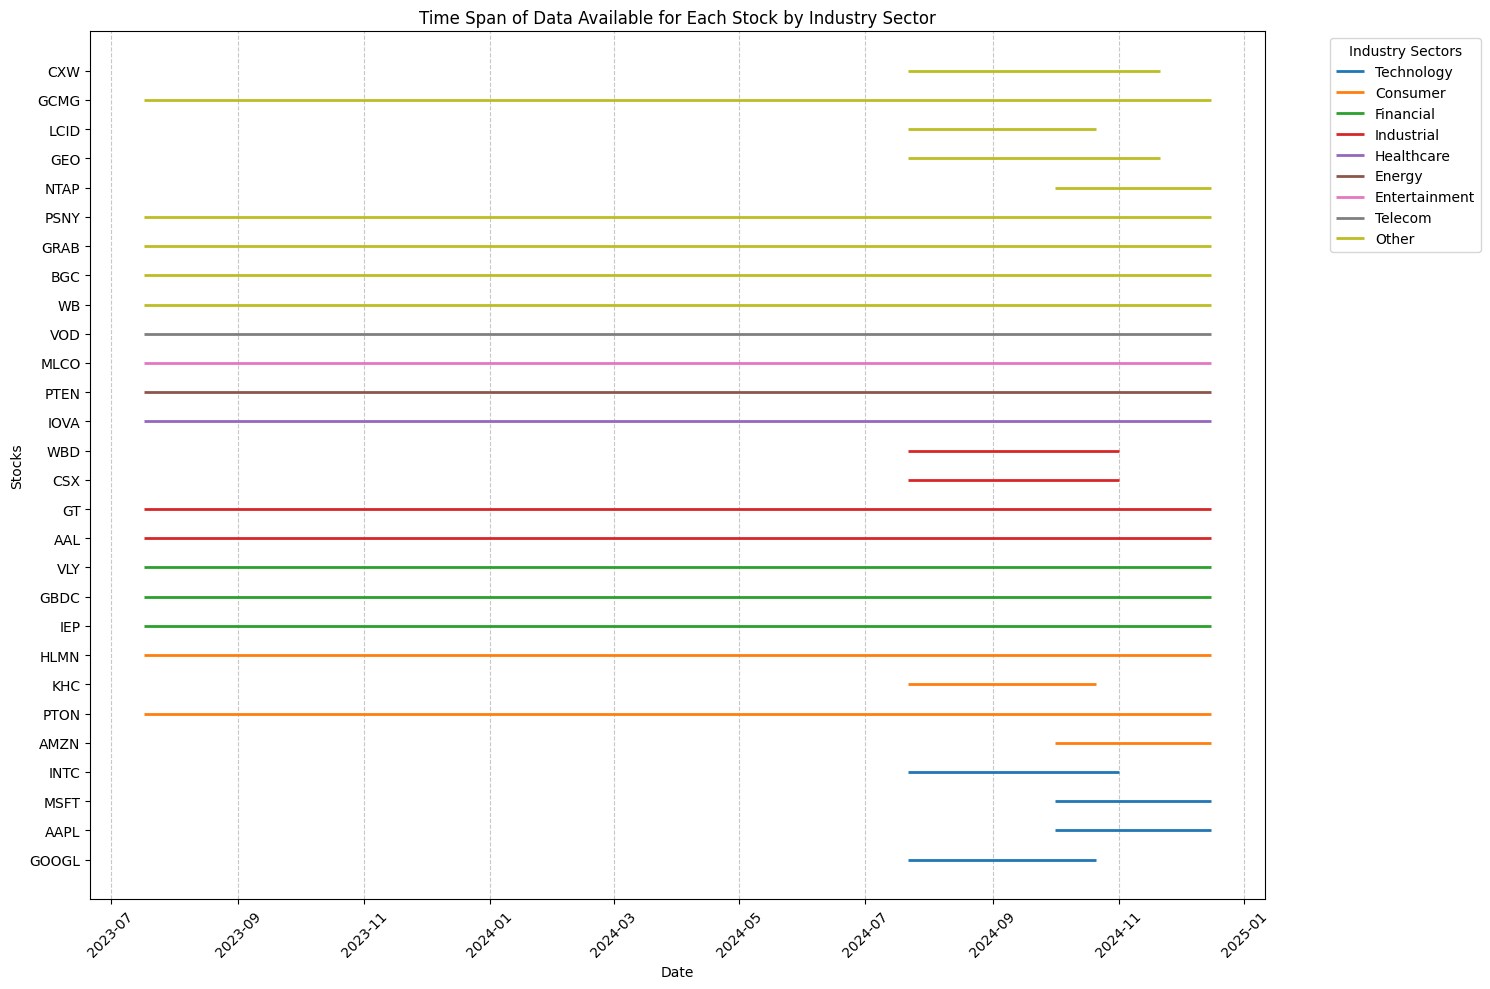
\includegraphics[width=0.53\textwidth]{time_expansion.png}
    \caption{Illustration de l'expansion temporelle des données, détaillée dans le notebook \texttt{timeexpansion.ipynb}.}
    \label{fig:time_expansion}
\end{figure}

\newpage
\section{Analyse de la stationnarité}

\subsection{Normalisation des données}

\begin{landscape}
\begin{table}[h!]
\centering
\begin{tabular}{|p{4cm}|p{6cm}|p{6cm}|}
\hline
\textbf{Étape} & \textbf{Description} & \textbf{Formulation mathématique} \\
\hline
Échantillonnage temporel & Les données sont échantillonnées à différentes échelles temporelles & $\{\text{30µs}, \text{100µs}, \text{1ms}, \text{10ms}, \text{100ms}, \text{1s}\}$ \\
\hline
Calcul des rendements & Pour chaque actif $i$, calcul des log-rendements du micro-price & $r_i(t) = \ln\left(\frac{P_i(t+\Delta t)}{P_i(t)}\right)$ \\
& où $P_i(t)$ est le microprix & $P_i(t) = \frac{P^a_i(t)V^b_i(t) + P^b_i(t)V^a_i(t)}{V^a_i(t) + V^b_i(t)}$ \\
\hline
Synchronisation des données & Les séries sont alignées temporellement et tronquées à la même longueur & - \\
\hline
Estimation des paramètres & Pour chaque paire d'actifs et chaque type de copule, estimation par maximum de vraisemblance & - \\
\hline
\end{tabular}
\caption{Étapes de normalisation des données}
\label{tab:norm_steps}
\end{table}
\end{landscape}


\subsection{Méthodologie}

\begin{landscape}
\begin{table}[h!]
\centering
\begin{tabular}{|p{4cm}|p{8cm}|p{8cm}|}
\hline
\textbf{Composante} & \textbf{Description} & \textbf{Formulation mathématique} \\
\hline
Test de stationnarité & Test de Dickey-Fuller augmenté (ADF) pour inférer la présence de racine unitaire dans le cas AR. L'hypothèse nulle $H_0: \gamma = 0$ correspond à la non-stationnarité. & $\Delta y_t = \alpha + \beta t + \gamma y_{t-1} + \sum_{i=1}^p \delta_i \Delta y_{t-i} + \epsilon_t$ \\
\hline
Détection des points de rupture & Méthode de clustering par window pour trouver les points de rupture dans la série temporelle. Les $\tau_k$ sont les points de rupture et $\bar{y}_k$ les moyennes locales. & $\min_{\tau_1,\ldots,\tau_K} \sum_{k=1}^{K+1} \sum_{t=\tau_{k-1}+1}^{\tau_k} \|y_t - \bar{y}_k\|^2 + \lambda K$ \\
\hline
Échelles temporelles analysées & Analyse effectuée sur quatre échelles temporelles différentes pour tous les stocks & $\{\text{100ms}, \text{1s}, \text{10s}, \text{60s}\}$ \\
\hline
\end{tabular}
\caption{Méthodologie d'analyse de la stationnarité}
\label{tab:stationarity_methodology}
\end{table}
\end{landscape}

\subsection{Résultats empiriques}

Les tests de stationnarité révèlent plusieurs caractéristiques importantes pour tous les stocks :


\begin{table}[h!]
\centering
\begin{tabular}{|p{2.5cm}|p{4cm}|p{4cm}|p{4cm}|}
\hline
\textbf{Échelle} & \textbf{Microscopique} (<100ms) & \textbf{Mésoscopique} (1s-10s) & \textbf{Macroscopique} (60s) \\
\hline
\textbf{Remarques} & 
    \begin{itemize}
        \item Forte non-stationnarité (p-value ADF > 0.05)
    \item Clusters de volatilité en début et fin de journée usuel en intraday.
\end{itemize} &
    \begin{itemize}
    \item Stationnarité par morceaux pour tous les actifs, on est entre l'influence de l'orderbook et l'influence macro
    \item Changements de régime moins fréquents mais significatifs de méta-ordre par exemple
\end{itemize} &
\begin{itemize}
        \item Stationnarité plus marquée
    \item Changements de régime principalement liés aux événements macroéconomiques, type annonce des taux FED le 18 Septembre 2024 à 16h GMT
\end{itemize} \\
\hline
\end{tabular}
\caption{Caractéristiques de stationnarité selon l'échelle temporelle}
\label{tab:stationarity_results}
\end{table}

\subsection{Exemple d'événement macroéconomique : Annonce du taux de chômage à 14h30 GMT}

Par exemple l'analyse du 8 août 2024 fournit un exemple particulièrement éclairant de l'interaction entre stationnarité et dépendance. Ce jour-là, l'annonce des chiffres du chômage a provoqué une réaction synchronisée sur l'ensemble du marché, illustrant parfaitement comment les événements macroéconomiques peuvent induire des changements de régime simultanés.

\begin{figure}[h!]
\centering
        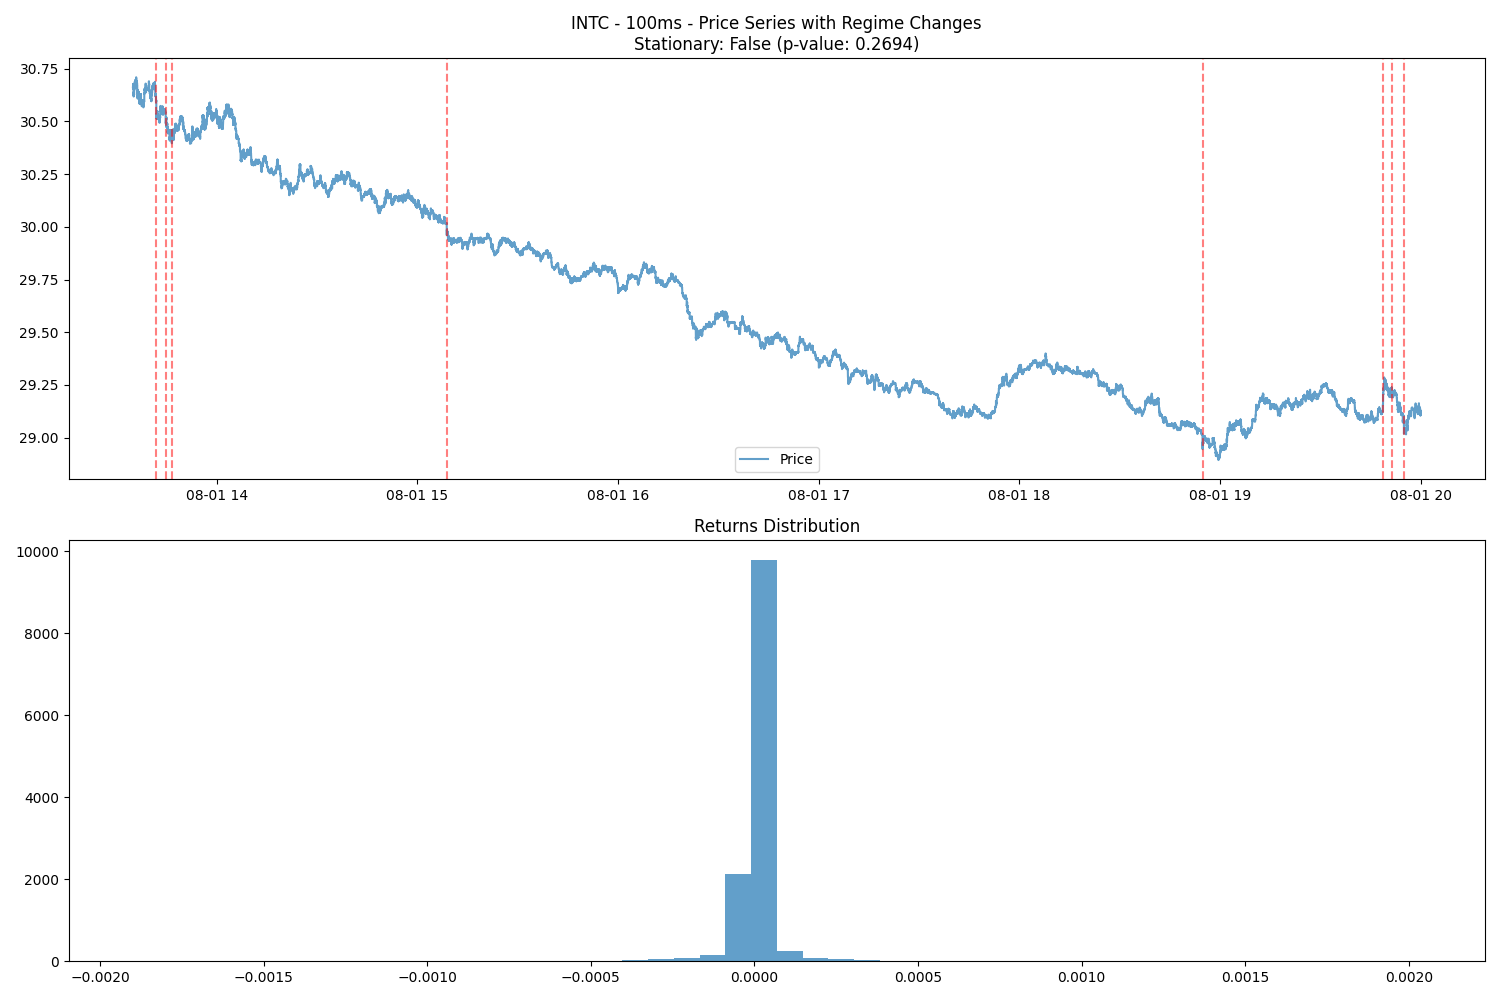
\includegraphics[width=0.3\textwidth]{INTC_2024-08-01_100ms.png}
        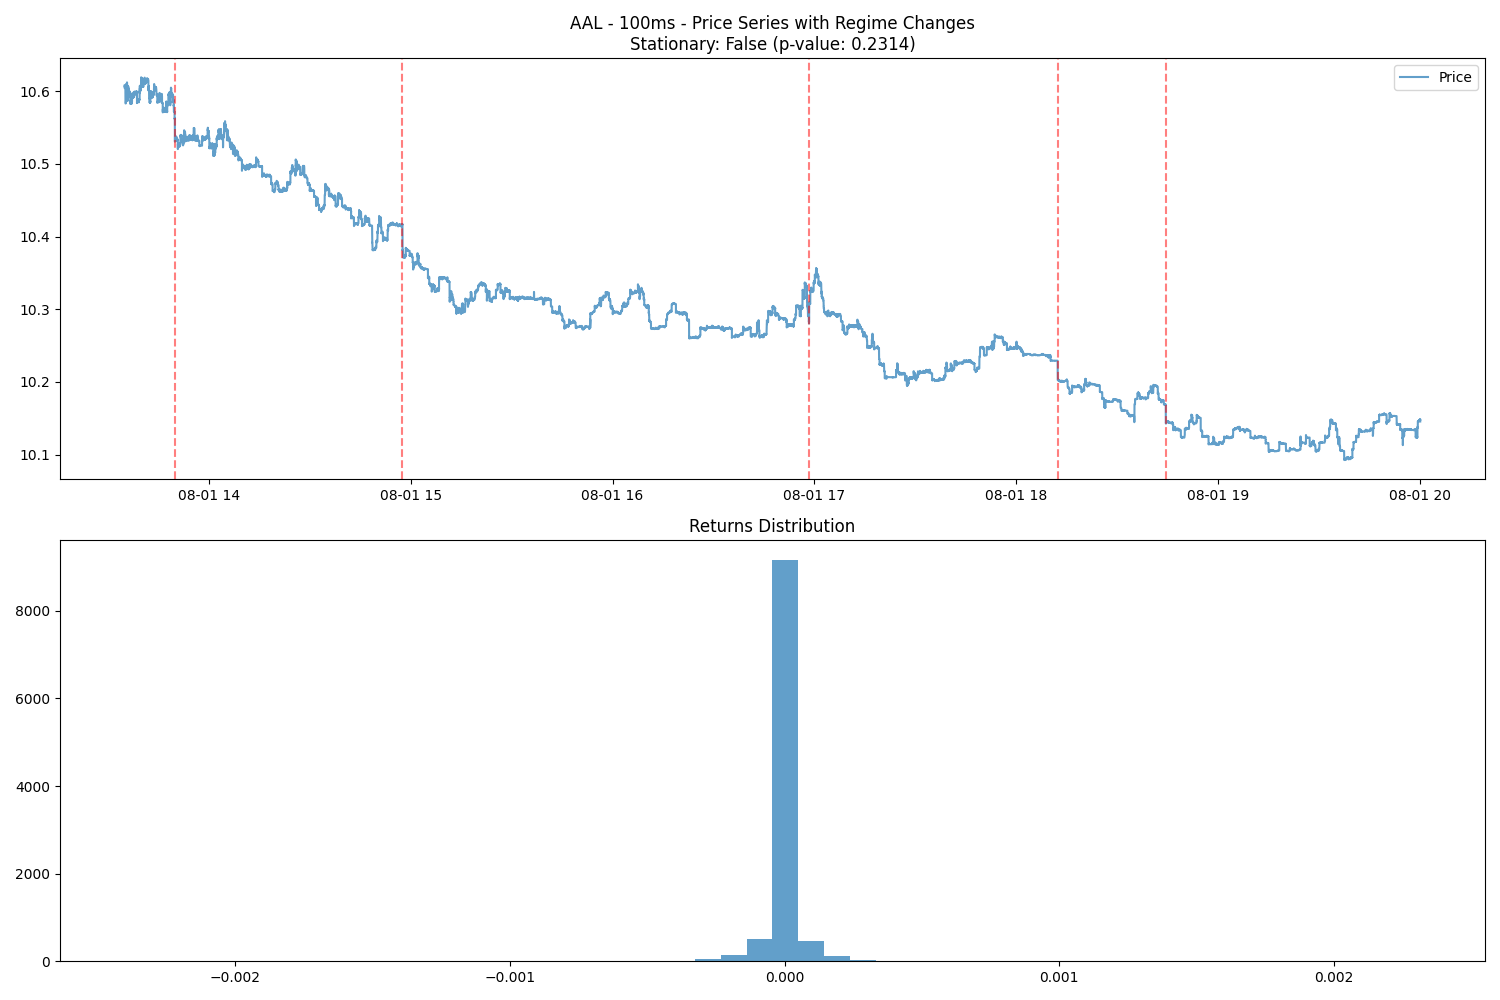
\includegraphics[width=0.3\textwidth]{AAL_2024-08-01_100ms.png}
        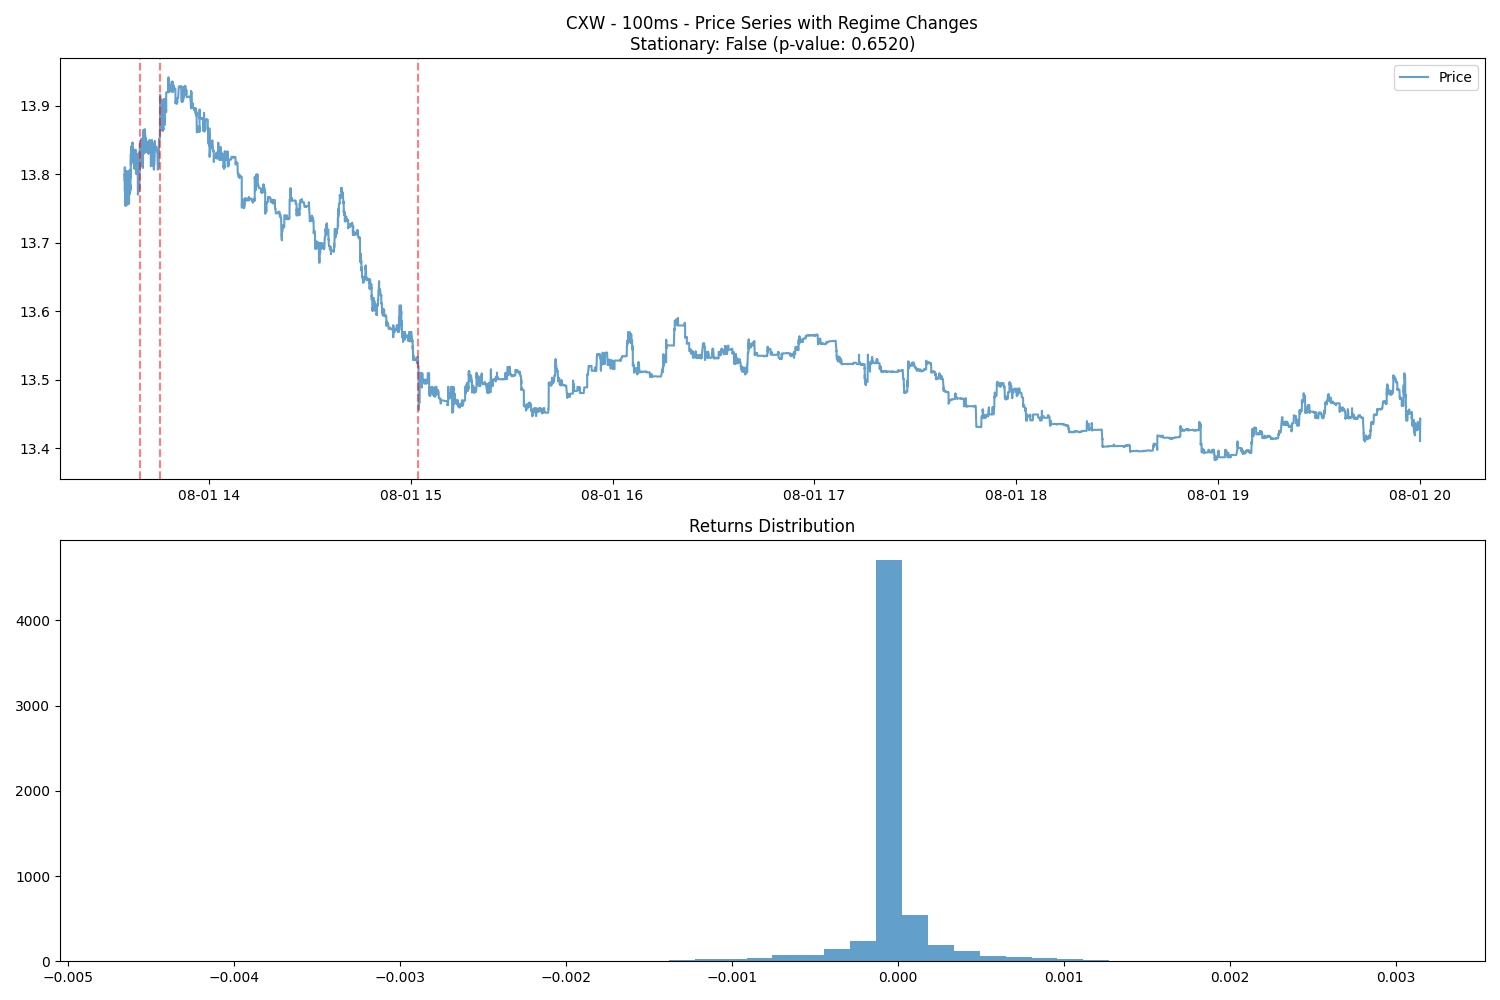
\includegraphics[width=0.3\textwidth]{CXW_2024-08-01_100ms.png}
        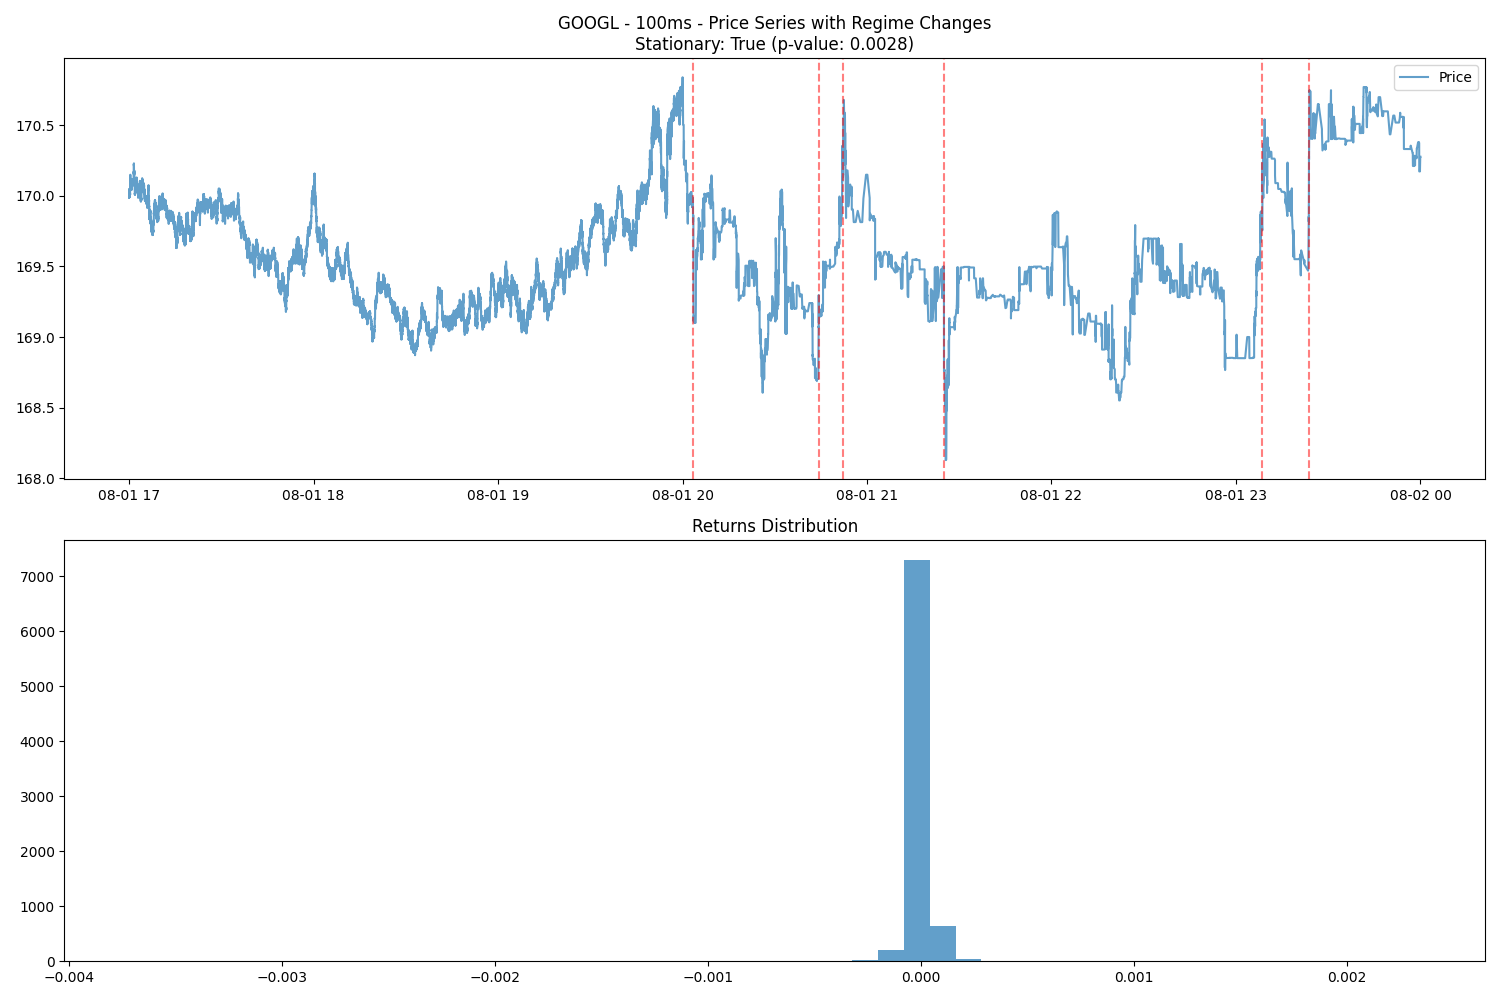
\includegraphics[width=0.3\textwidth]{GOOGL_2024-08-01_100ms.png}
    \caption{Analyse de stationnarité pour INTC, AAL, CXW et GOOGL le 8 août 2024 à l'échelle de 100ms et en temps GMT. Les lignes verticales rouges indiquent les changements de régime détectés.
    Le dataset GOOGL était shifté de 6h pour correspondre au temps GMT, donc pic à 20h sur le graphe}
    \label{fig:stationarity_unemployment}
\end{figure}

Cette journée montre plusieurs phénomènes importants :

\begin{itemize}
        \item Les rendements montrent une partie fat tail (l'échelle matplotlib s'ajuste automatiquement) avec un certain nombre de valeurs extrêmes. On ne calcule pas de Hill ici car l'analyse est faite plus tard mais on le voit apparaitre directement visuellement ce qui est rassurant.
        \item Les rendements montrent aussi qu'une partie de la tendance est expliquée par les variations tick-by-tick intraday (2ème plus grosse barre de l'histogramme), ce qui suggère l'explication de la tendance par des méta-ordres (et donc d'une imbalance bid-ask moyenne non nulle)
        \item Les changements de régime sont traités comme des points de rupture distincts, on les voit particulièrement en début et fin d'activité  du marché (d'où la suppression générale de la 1ère/dernière heure d'activité)
\end{itemize}


Cette observation est fondamentale car elle démontre que l'apparente indépendance des rendements à haute fréquence n'est pas incompatible avec l'existence de mouvements coordonnés du marché. 
Et donc la stationnarité locale est préservée précisément parce que ces événements sont traités comme des points de rupture plutôt que comme des variations continues du processus.
En tout cas, on s'intéressera dans le futur à la description haute fréquence de cet événement et son explication en termes de méta-ordres (et donc d'imbalance) par exemple. 
Nous avons aussi intégré des fit ARMA/GARCH sur les rendements pour trouver les changepoints et interpréter une partie du Hurst mais cette analyse sera détaillée dans le futur sur le github puisque 13 pages sont trop courtes pour tout présenter.

Pour l'heure, maintenant que l'on a trouvé des stocks et journées plutôt stationnaires, on peut maintenant mieux ajuster un modèle brownien fractionnaire le plus indépendant possible du sampling time.


\section{Modélisation de Hurst et extraction de la volatilité}

\subsection{Présentation du modèle de Hurst}

L'exposant de Hurst, noté H, est un indicateur statistique qui permet de caractériser la régularité d'un processus, notamment en termes de persistance ou d'anti-persistance. Dans le contexte HFT, cet exposant nous permet d'analyser la mémoire du processus de prix et de quantifier sa prédictibilité à différentes échelles de temps.

Pour une série temporelle \(X(t)\), l'exposant de Hurst H est défini par la relation:

\[
E[|X(t+\tau) - X(t)|^q] \propto \tau^{qH}
\]

où \(\tau\) représente l'intervalle de temps considéré. L'interprétation de H est la suivante:
\begin{itemize}
    \item H = 0.5 : Mouvement brownien standard (marche aléatoire)
    \item H > 0.5 : Persistance (tendance à maintenir sa direction)
    \item H < 0.5 : Anti-persistance (tendance à s'inverser)
\end{itemize}

En étant en haute fréquence, on se place d'ores et déjà dans un modèle Bachelier puisque nous sommes à la limite de la fusion variation tick-by-tick -> variation continue.
Nous n'utilisons pas les méthodes de calcul stochastique/MLE vu dans le cours de Mr. Kébaier pour l'instant, cela sera fait dans le futur, nous nous cantonons au modèle Bachelier avec timestamps irréguliers.
On peut donc estimer très simplement H avec un OLS des log-coordonnées.

\subsection{Procédure d'extraction de la volatilité}

\begin{landscape}
\begin{table}[h!]
\centering
\begin{tabular}{|p{0.25\linewidth}|p{0.75\linewidth}|}
\hline
\textbf{Étape} & \textbf{Description} \\
\hline
1. Calcul du temps moyen & Détermination de \(\Delta t_{avg}\) entre les changements de prix \\
\hline
2. Échantillonnage multi-échelle & Processus de prix échantillonné aux échelles temporelles: \[\{\Delta t_{avg}, 5\Delta t_{avg}, 10\Delta t_{avg}, ..., 3000\Delta t_{avg}\}\] \\
\hline
3. Normalisation des variations & Pour chaque échelle \(\tau\), calcul des variations normalisées: \[\Delta P_{\tau} = \frac{P(t+\tau) - P(t)}{\sigma}\] où \(\sigma\) est la moyenne du spread bid-ask \\
\hline
4. Estimation de la volatilité & Application du modèle de Bachelier: \[\sigma_{\tau} = \frac{|\Delta P_{\tau}|}{\sqrt{\tau}}\] \\
\hline
\end{tabular}
\caption{Procédure systématique d'extraction de la volatilité à différentes échelles temporelles}
\label{tab:volatility_extraction}
\end{table}
\end{landscape}


\begin{figure}[H]
    \centering
    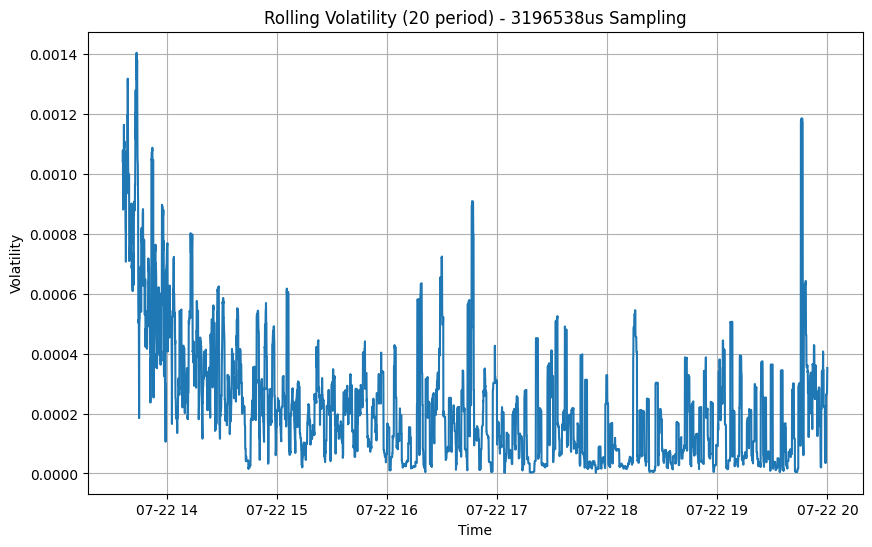
\includegraphics[width=0.8\textwidth]{rollingvola.png}
    \caption{Profil de vol intraday (non normalisée par le spread bid-ask moyen) sur une journée, on voit la faible régularité typique d'un Hurst petit avec de nombreux spikes, et un début/fin de journée bien volatil}
    \label{fig:jump_example_1}
\end{figure}

\subsection{Résultats empiriques}

On choisit par exemple l'actif WBD pour illustrer les résultats, car il présente une stationnarité marquée sur la période considérée. Notre approche est systématique est runnable sur tout actif.
L'analyse des données pour l'actif WBD révèle plusieurs caractéristiques intéressantes:

\begin{itemize}
    \item Le temps moyen entre les changements de prix est de l'ordre de \(10^{-3}\) secondes
    \item La distribution des temps d'arrivée présente une queue lourde, caractéristique des processus de Poisson inhomogènes
    \item La volatilité normalisée \(\sigma_{\tau}\) montre une dépendance en loi de puissance par rapport à l'échelle de temps \(\tau\)
\end{itemize}
\begin{table}[h!]
\centering
\begin{tabular}{|c|c|}
\hline
\textbf{Échelle temporelle (µs)} & \textbf{Exposant de Hurst (H)} \\
\hline
2 041 & 0.229 \\
10 207 & 0.250 \\
20 415 & 0.268 \\
61 247 & 0.270 \\
204 157 & 0.284 \\
2 041 576 & 0.285 \\
6 124 728 & 0.297 \\
20 415 762 & 0.278 \\
61 247 288 & 0.310 \\
204 157 627 & 0.329 \\
\hline
\end{tabular}
\caption{Estimations de l'exposant de Hurst pour WBD à différentes échelles temporelles}
\label{tab:hurst_exponents}
\end{table}

Cette anti-persistance (H < 0.5) suggère une forte tendance à la réversion vers la moyenne à court terme, caractéristique des marchés dominés par des market makers et des stratégies de trading haute fréquence. Plusieurs observations importantes émergent :

\begin{itemize}
    \item À l'échelle microscopique (< 100 ms), H ≈ 0.23-0.27, indiquant une forte anti-persistance, nous ne sommes pas au niveau de H ≈ 0.1 comme esperé mais pour des hypothèses simplistes et un traitement systématique et non 
    \item Aux échelles intermédiaires (100 ms - 60 s), H augmente progressivement jusqu'à ≈ 0.33
\end{itemize}

Cette structure multi-échelle de l'exposant de Hurst reflète différents régimes de marchés et acteurs :
\begin{itemize}
    \item L'anti-persistance à très court terme est cohérente avec le comportement de bounce du spread bid-ask
    \item L'augmentation de H aux échelles intermédiaires suggère donc l'influence croissante des tendances directionnelles, où l'hypothèse Bachelier n'est plus respectéé.
\end{itemize}

\begin{figure}[h!]
    \centering
        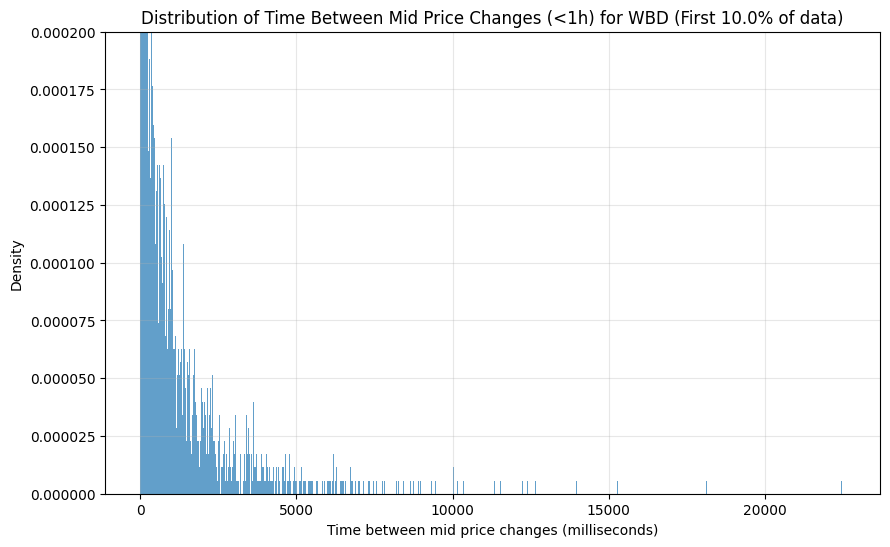
\includegraphics[width=0.53\textwidth]{arrivaltimewbd.png}
    \caption{Distribution des temps d'arrivée entre les changements de prix pour WBD. Un de nos meilleurs plot : La queue lourde observée (fat tail) est caractéristique d'un processus avec meta-orders, conformément aux travaux de Rosenbaum qui prédisent cette distribution en loi de puissance pour les arrivées.}
    \label{fig:arrival_times_wbd}
\end{figure}


On sait aussi maintenant que le processus est stationnaire, donc on peut faire l'autocorrélation sur le processus stationnaire, qui nous donne un résultat montrant en partie
(décroissance linéaire à taux faible et constant en échelle log) la persistance de la volatilité. En ayant une décroissance lente (pas aussi lente que linéaire dans le cas mouvement brownien fractionnaire)
on peut en conclure que le processus est assez persistant.

\begin{figure}[h!]
    \centering
        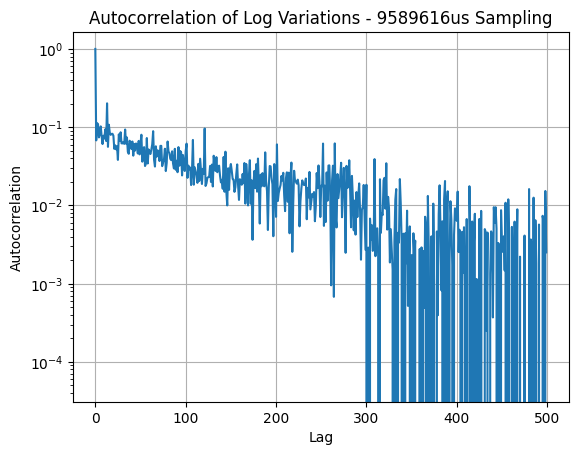
\includegraphics[width=0.53\textwidth]{autocorr.png}
    \caption{Fonction d'autocorrélation des rendements pour WBD. La décroissance lente de l'autocorrélation confirme la présence de mémoire longue significative dans la série temporelle des rendements, conformément à l'hypothèse d'efficience du marché à ces échelles de temps.}
    \label{fig:autocorr_wbd}
\end{figure}



Dans le futur, nous souhaitons mettre en place des approches d'estimation plus robustes \cite{chong2024minimax, chong2024clt} pour estimer H, et les comparer aux approche wavelets plus anciennes. 



\begin{figure}[h!]
    \centering
        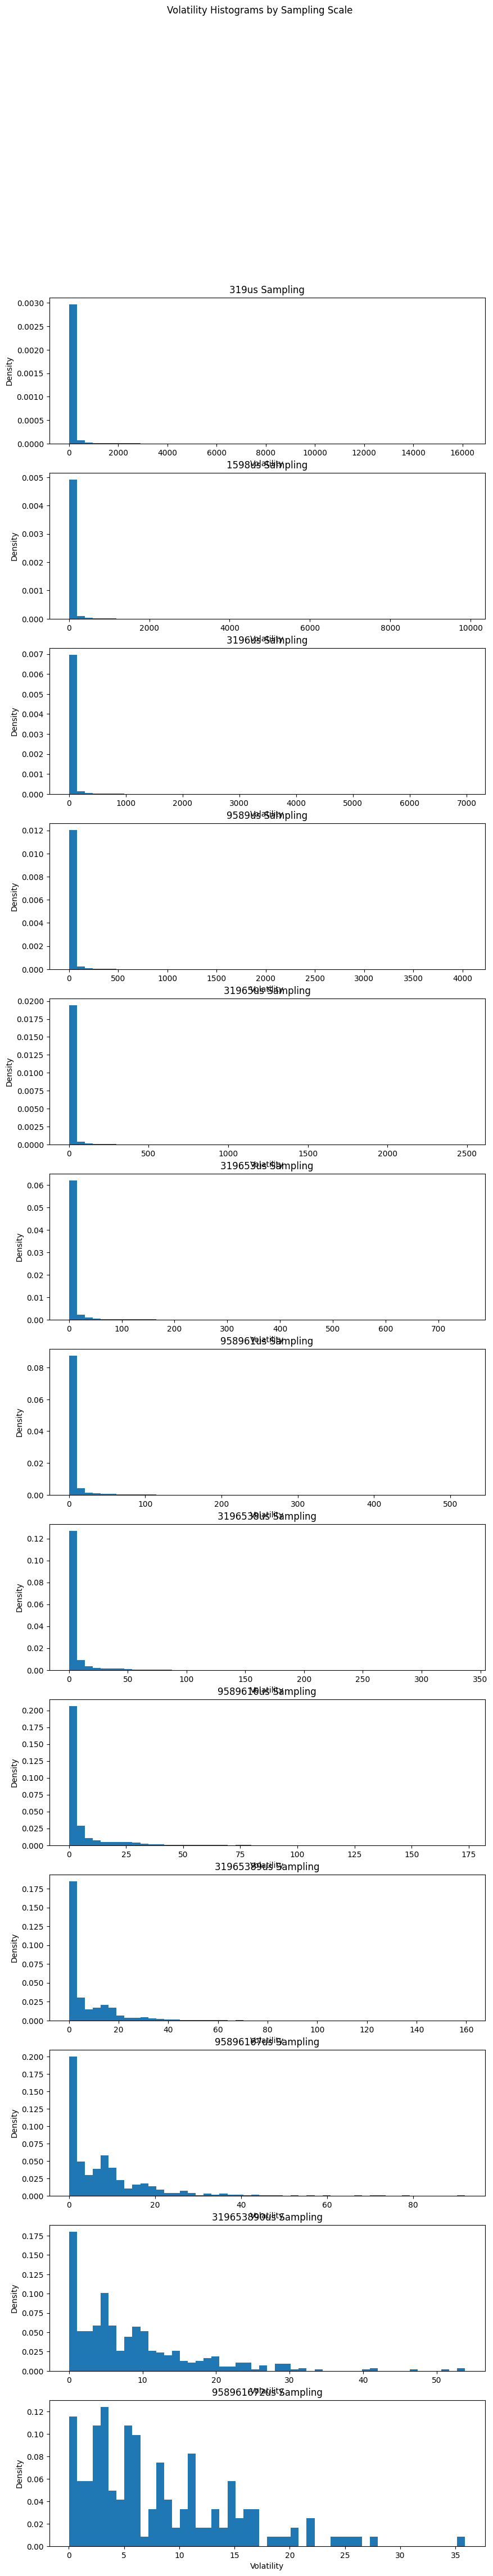
\includegraphics[width=0.53\textwidth]{wbd_logvar.png}
    \caption{Distribution des log-variations non spread-normalisées de prix sur l'échelle 1m-10m-1h pour WBD. L'écart significatif par rapport à la distribution normale (pointillés) confirme la nature leptokurtique des rendements haute fréquence.}
    \label{fig:log_variations_wbd}
\end{figure}
\begin{figure}[h!]
    \centering
    \begin{subfigure}[b]{0.48\textwidth}
        \includegraphics[width=\textwidth]{output1.png}
    \end{subfigure}
    \hfill
    \begin{subfigure}[b]{0.48\textwidth}
        \includegraphics[width=\textwidth]{output2.png}
    \end{subfigure}
    \caption{Histogrammes de la vol pour WBD. Les distributions sont heavy tailed, on a donc une probabilité accrue d'événements extrêmes par rapport à une distribution gaussienne.}
    \label{fig:volatility_hist}
\end{figure}


\subsection{Analyse multi-échelle des distributions de rendements}

L'étude des distributions de rendements à différentes échelles temporelles révèle l'évolution de la structure statistique des prix en fonction de l'horizon d'observation.

\subsubsection{Estimation des queues de distribution des rendements}

L'analyse des queues de distribution des rendements est cruciale pour comprendre le comportement des événements extrêmes dans les marchés financiers. Nous avons utilisé plusieurs approches complémentaires pour caractériser ces queues :

\paragraph{Estimation de Hill}
Pour les rendements normalisés $r_t$, nous avons estimé l'indice de queue $\alpha$ via la méthode de Hill :

\begin{equation}
\hat{\alpha}_k = \left(\frac{1}{k} \sum_{i=1}^k \log \frac{X_{(i)}}{X_{(k+1)}}\right)^{-1}
\end{equation}

où $X_{(i)}$ sont les statistiques d'ordre des valeurs absolues des rendements. Les résultats généraux montrent :

Afin d'obtenir des estimations cohérentes, on estime le returns à différentes échelles temporelles (m pour minutes, h pour heure)
Notamment, à partir de l'échèle seconde, les effets des variations tick by tick se font sentir (voir figure des rendements IEP)
Il a donc fallu trouver un compromis entre expressivité du sampling et quantité de données pour une estimation fat tail robuste avec peu de données comme vue en cours.
On applique donc strictement la méthode de Hill en restant proche des hypothèses du cours.



\begin{table}[H]
\centering
\begin{tabular}{lcccc}
\toprule
Actif-Échelle & $\alpha$ global & $\alpha$ queue gauche & $\alpha$ queue droite & p-value KS \\
\midrule
KHC-10m & 3.02 & 3.02 & 3.00 & 0.12 \\
\midrule
CXW-5m & 2.66 & 2.61 & 2.70 & 0.99 \\
CXW-30m & 2.70 & 2.61 & 2.77 & 0.40 \\
CXW-1h & 2.64 & 2.65 & 2.71 & 0.63 \\
\midrule
WBD-20m & 2.73 & 2.83 & 2.63 & 0.61 \\
\midrule
IEP-5m & 2.58 & 2.59 & 2.56 & 0.38 \\
IEP-10m & 2.54 & 2.60 & 2.47 & 0.37 \\
IEP-20m & 2.52 & 2.46 & 2.61 & 0.08 \\
IEP-30m & 2.47 & 2.44 & 2.50 & 0.88 \\
\bottomrule
\end{tabular}
\caption{Estimations détaillées de l'indice de queue par la méthode de Hill à différentes échelles temporelles}
\label{tab:hill_detail_moved}
\end{table}

Plusieurs observations importantes émergent de cette analyse multi-échelle des exposants :

\begin{itemize}
    \item L'actif KHC présente les queues les plus fines (α ≈ 3.0), indiquant une moindre propension aux événements extrêmes
    \item Les actifs IEP et CXW affichent les queues les plus épaisses (α ≈ 2.5-2.7), suggérant une probabilité plus élevée d'événements extrêmes
    \item On observe une tendance générale à la diminution de l'exposant α avec l'augmentation de l'échelle temporelle pour IEP (de 2.58 à 5m à 2.47 à 30m). L'exposant est très rassurant par rapport à ce qui est courant en HFT \cite{saddier2024bayesiantheorymarketimpact}
    \item La p-value du test de Kolmogorov-Smirnov reste élevée pour toutes les échelles, confirmant l'excellente adéquation du modèle en loi de puissance
    \item Les différences entre les queues gauche et droite sont généralement modérées, mais certains actifs (WBD, IEP-10m) présentent une asymétrie plus marquée
\end{itemize}
Ces résultats confirment que les rendements financiers suivent universellement des lois de puissance avec des exposants caractéristiques dans la plage 2.4-3.1, significativement inférieurs aux valeurs qu'impliquerait un modèle gaussien. On ajuste également des power-law sur les queues de distribution, l'estimation ayant été réalisée par maximum de vraisemblance sur des fonctions du type lorentzienne $\frac{a}{b+x^c}$ avec un seuil adaptatif. Les résultats montrent une excellente adéquation avec les lois de puissance, avec des exposants $\alpha$ cohérents avec l'estimation de Hill. Par ailleurs, nous aurions pu mettre en oeuvre un Q-Q plot, puis fitter $\hat \alpha$ avec son équvalent théorique fat-tail $\alpha$ vs gaussian, mais cela se fera dans la suite du projet (sur github). Nous souhaitions principalement fabriquer des plots avec un fit fat-tail marquant. La nature même d'un histogramme automatiquement décentré et visible de loin (donc scale-invariant) avec quelques samples très extrêmes montre la nature fat-tail en plus de l'estimation de Hill.

\subsubsection{Rendements de CXW à différentes échelles}

\begin{figure}[H]
    \centering
    \begin{subfigure}[b]{0.45\textwidth}
        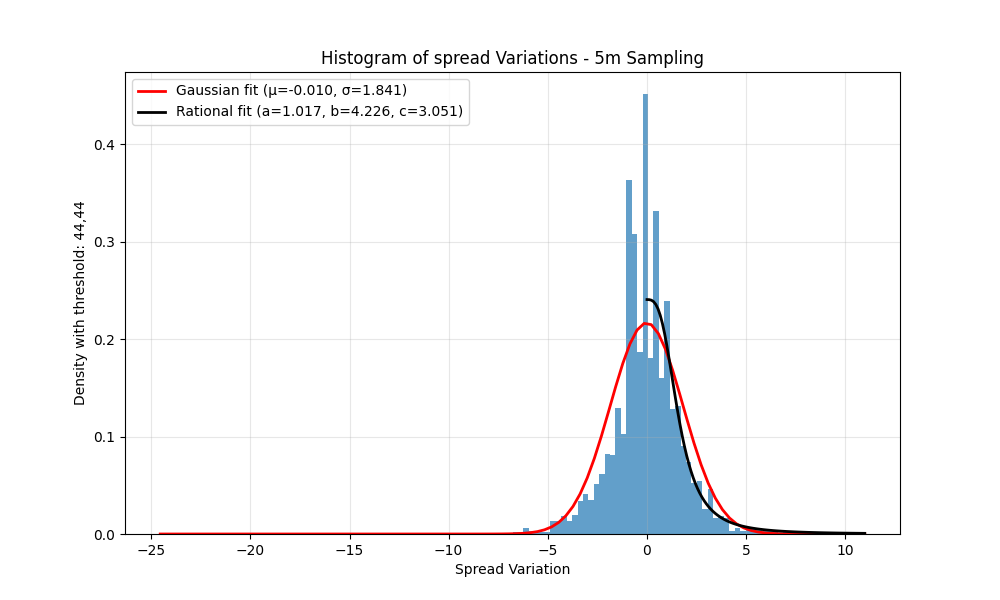
\includegraphics[width=\textwidth]{CXW_5m_returns_histogram.png}
        \caption{Distribution des rendements à 5 minutes}
        \label{fig:CXW_5m_moved}
    \end{subfigure}
    \hfill
    \begin{subfigure}[b]{0.45\textwidth}
        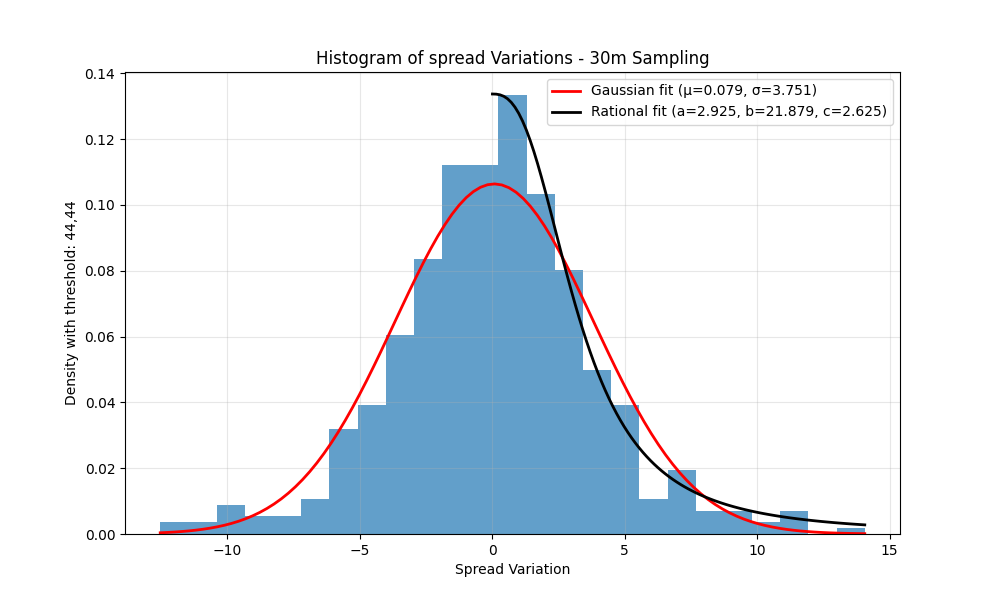
\includegraphics[width=\textwidth]{CXW_30m_returns_histogram.png}
        \caption{Distribution des rendements à 30 minutes}
        \label{fig:CXW_30m_moved}
    \end{subfigure}
    \caption{Distributions des rendements pour CXW à 5 et 30 minutes}
\end{figure}
    
\begin{figure}[H]
    \centering
    \begin{subfigure}[b]{0.45\textwidth}
        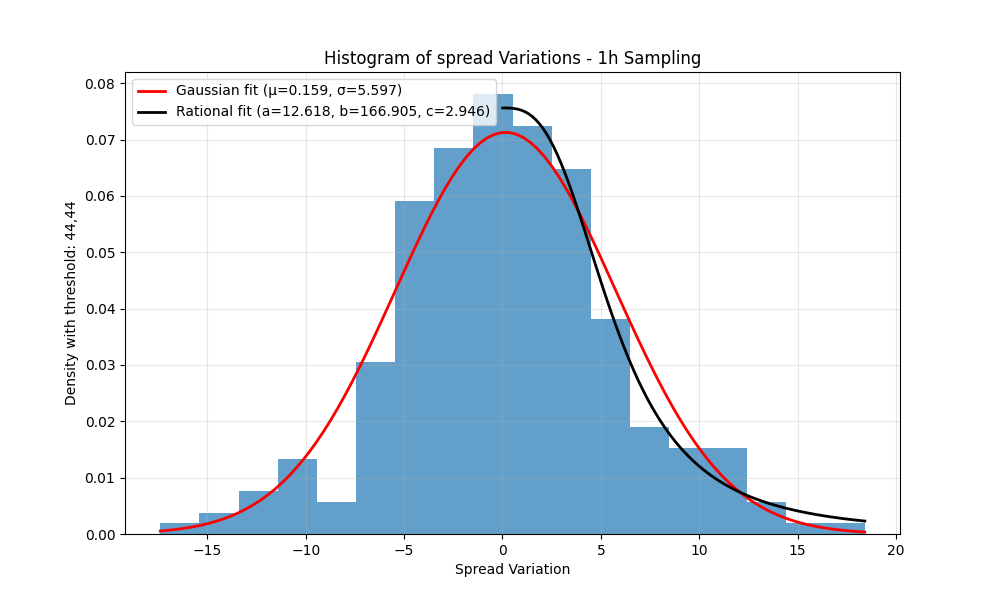
\includegraphics[width=\textwidth]{CXW_1h_returns_histogram.png}
        \caption{Distribution des rendements à 1 heure}
        \label{fig:CXW_1h_moved}
    \end{subfigure}
    \caption{Distribution des rendements pour CXW à 1 heure. Les ajustements en loi de puissance (courbes rouges) montrent des exposants caractéristiques entre 3.2 et 3.6, cohérents avec les travaux théoriques sur les marchés financiers. Notons que l'épaisseur des queues diminue légèrement avec l'allongement de l'échelle temporelle, suggérant un retour progressif vers la normalité. Les spikes sur l'histogramme sont dûs à la discrétisation en tick car IEP est un actif à gros tick de spread moyen proche de 1}
    \label{fig:CXW_multi_scale_moved}
\end{figure}

\subsubsection{Rendements de IEP à différentes échelles}

\begin{figure}[H]
    \centering
    \begin{subfigure}[b]{0.45\textwidth}
        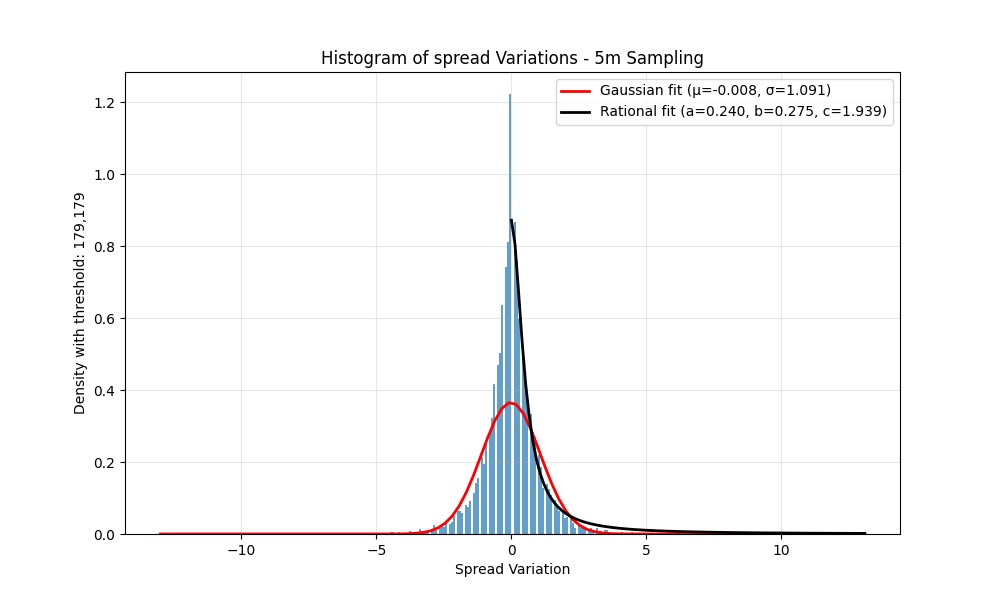
\includegraphics[width=\textwidth]{IEP_5m_returns_histogram.png}
        \caption{Distribution des rendements à 5 minutes}
        \label{fig:IEP_5m_moved}
    \end{subfigure}
    \hfill
    \begin{subfigure}[b]{0.45\textwidth}
        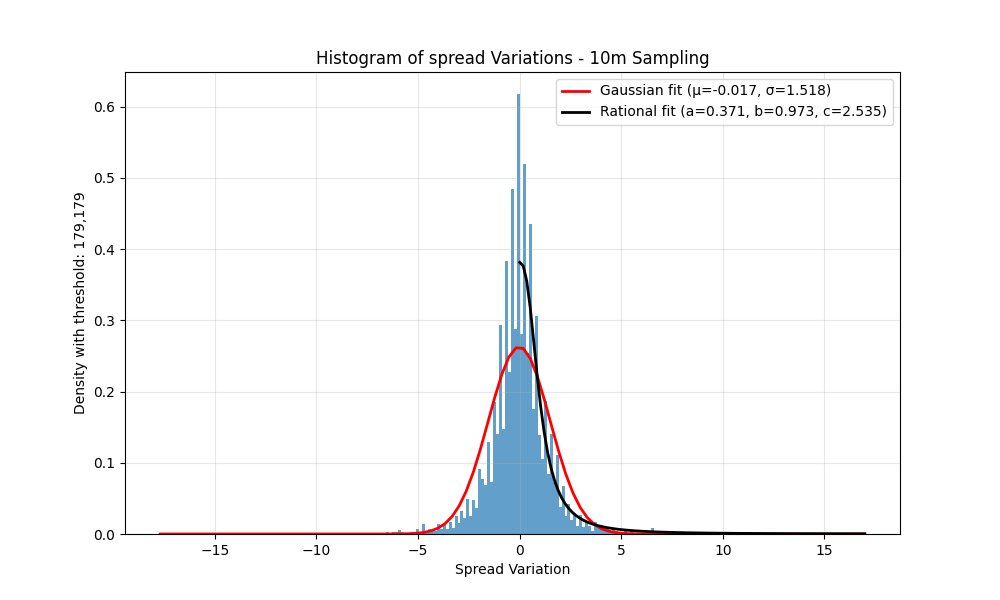
\includegraphics[width=\textwidth]{IEP_10m_returns_histogram.png}
        \caption{Distribution des rendements à 10 minutes}
        \label{fig:IEP_10m_moved}
    \end{subfigure}
    \caption{Distributions des rendements pour IEP à 5 et 10 minutes}
\end{figure}
    
\begin{figure}[H]
    \centering
    \begin{subfigure}[b]{0.45\textwidth}
        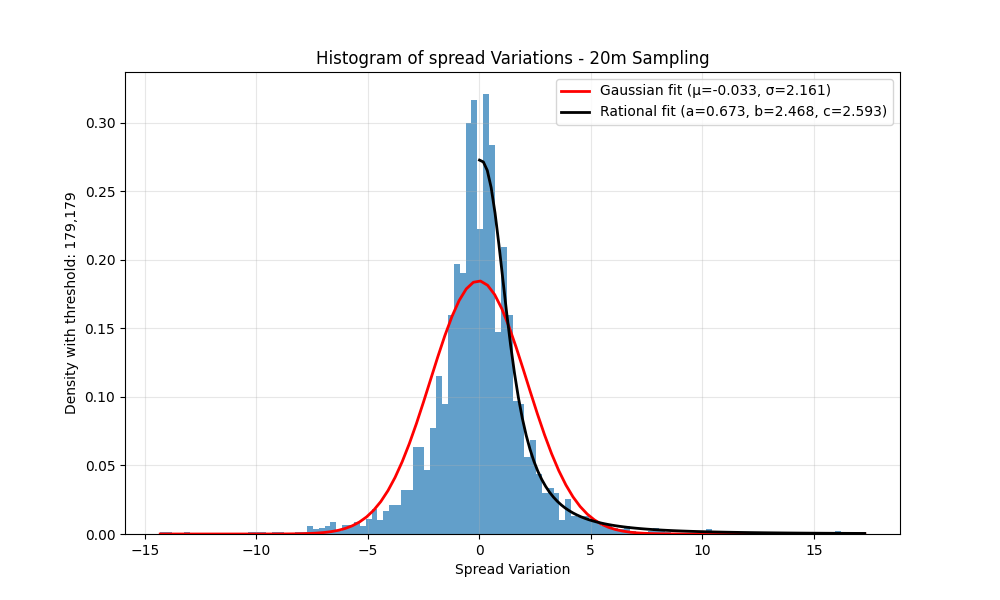
\includegraphics[width=\textwidth]{IEP_20m_returns_histogram.png}
        \caption{Distribution des rendements à 20 minutes}
        \label{fig:IEP_20m_moved}
    \end{subfigure}
    \hfill
    \begin{subfigure}[b]{0.45\textwidth}
        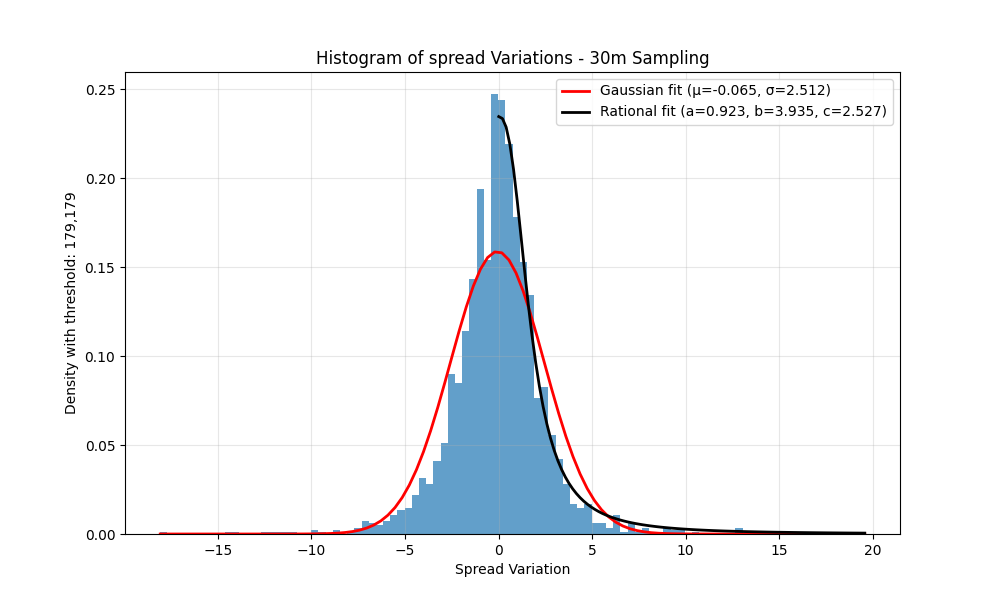
\includegraphics[width=\textwidth]{IEP_30m_returns_histogram.png}
        \caption{Distribution des rendements à 30 minutes}
        \label{fig:IEP_30m_moved}
    \end{subfigure}
    \caption{Distributions des rendements pour IEP à 20 et 30 minutes. Les distributions suivent des lois de puissance avec des exposants qui varient entre 3.0 et 3.5 selon l'échelle. Cette structure en loi de puissance est caractéristique des systèmes complexes auto-organisés et reflète le comportement collectif des acteurs du marché.}
    \label{fig:IEP_multi_scale_moved}
\end{figure}

\subsubsection{Rendements de WBD et KHC}

\begin{figure}[H]
    \centering
    \begin{subfigure}[b]{0.45\textwidth}
        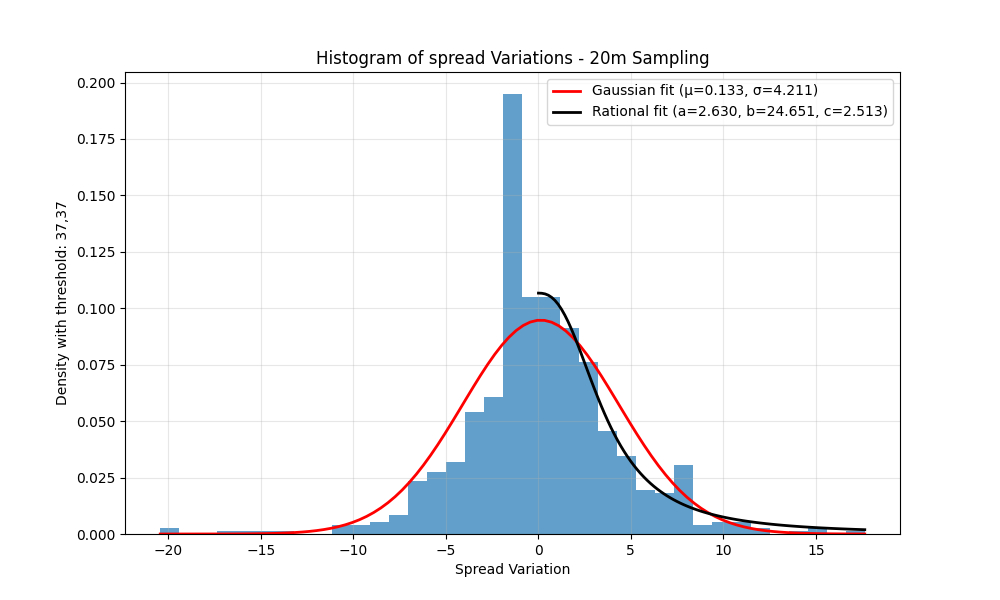
\includegraphics[width=\textwidth]{WBD_20m_returns_histogram.png}
        \caption{Distribution des rendements de WBD à 20 minutes}
        \label{fig:WBD_20m_moved}
    \end{subfigure}
    \hfill
    \begin{subfigure}[b]{0.45\textwidth}
        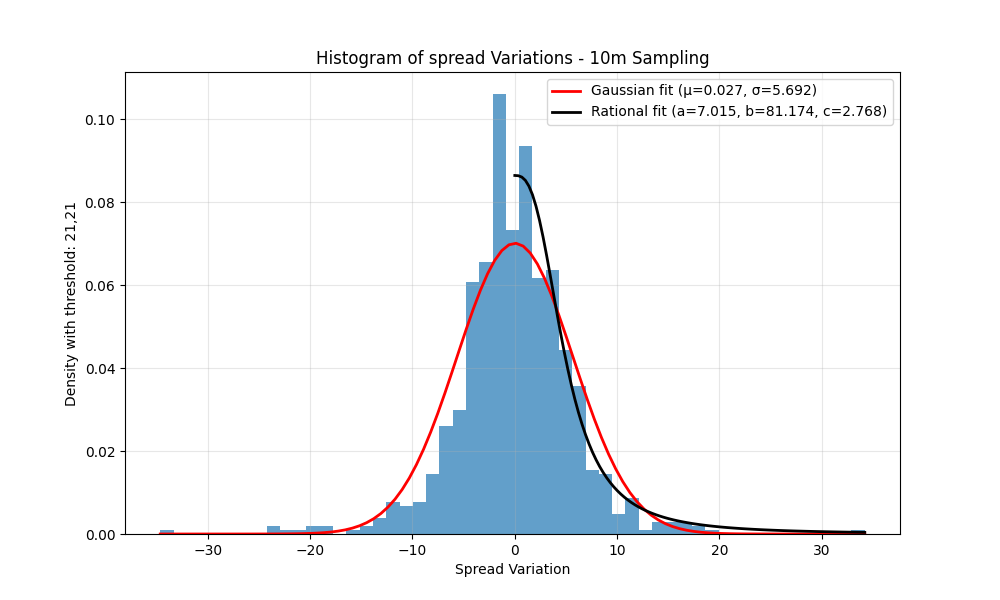
\includegraphics[width=\textwidth]{KHC_10m_returns_histogram.png}
        \caption{Distribution des rendements de KHC à 10 minutes}
        \label{fig:KHC_10m_moved}
    \end{subfigure}
    \caption{Comparaison des distributions de rendements pour WBD et KHC. Malgré des secteurs d'activité différents, les deux actifs présentent des distributions similaires en loi de puissance, suggérant un mécanisme universel sous-jacent dans la formation des prix sur les marchés financiers.}
    \label{fig:WBD_KHC_returns_moved}
\end{figure}


Ceci mis en place, on sait maintenant que nos returns sont de carré intégrable au moins ! Le cours fait aussi état d'une remarque importante : l'hypothèse $L^2$ est importante pour donner un sens aux corrélations !

Ainsi, on sait que l'on peut calculer des corrélations entre returns en pouvant donner une vraie interprétation puisque toutes les hypothèses ($n \gg p$ et $L^2$) sont respectées.

\section{Structure de corrélation entre actifs}

Ainsi, l'analyse des corrélations entre les rendements des différents actifs est ici calculée à différentes échelles temporelles, et révèle une partie de la structure de dépendance du marché. 
Nous examinons ici par exemple les matrices de corrélation pour la journée du 22 juillet 2024 aux échelles 10ms, 1s et 10s. Le notebook data/curating/correlation.ipynb permet de reproduire les expériences.

\begin{figure}[H] % Use H to place figures more strictly here
    \centering
        \begin{subfigure}[b]{0.32\textwidth} % Ajustement de la largeur pour alignement horizontal
            \centering % Centrer l'image dans la subfigure
            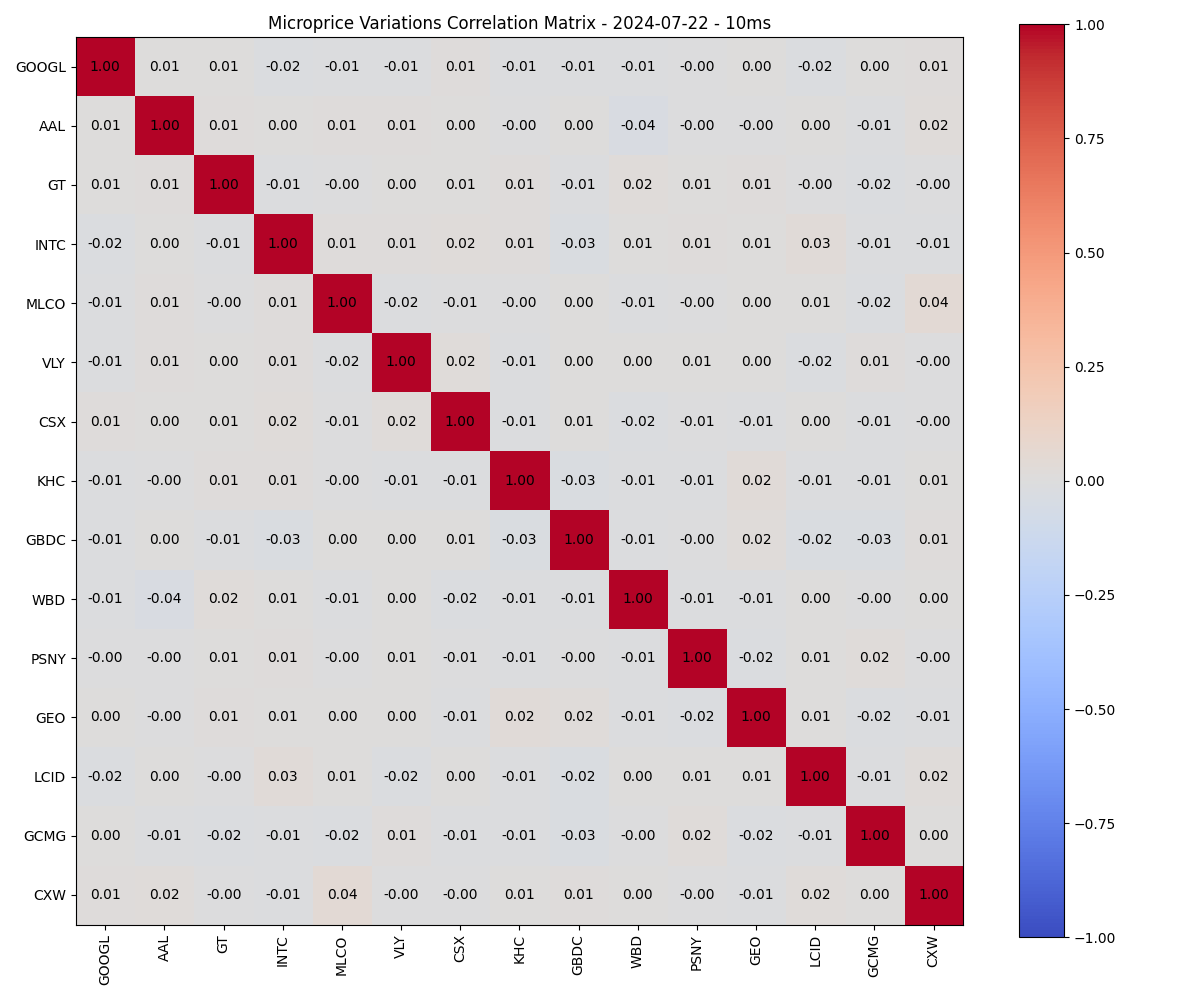
\includegraphics[width=\textwidth]{variations_matrix_2024-07-22_10ms.png} % Image prend toute la largeur de la subfigure
        \caption{Échelle 10ms}
        \label{fig:corr_10ms}
    \end{subfigure}
        \hfill % Espace horizontal flexible
        \begin{subfigure}[b]{0.32\textwidth} % Ajustement de la largeur pour alignement horizontal
            \centering % Centrer l'image dans la subfigure
            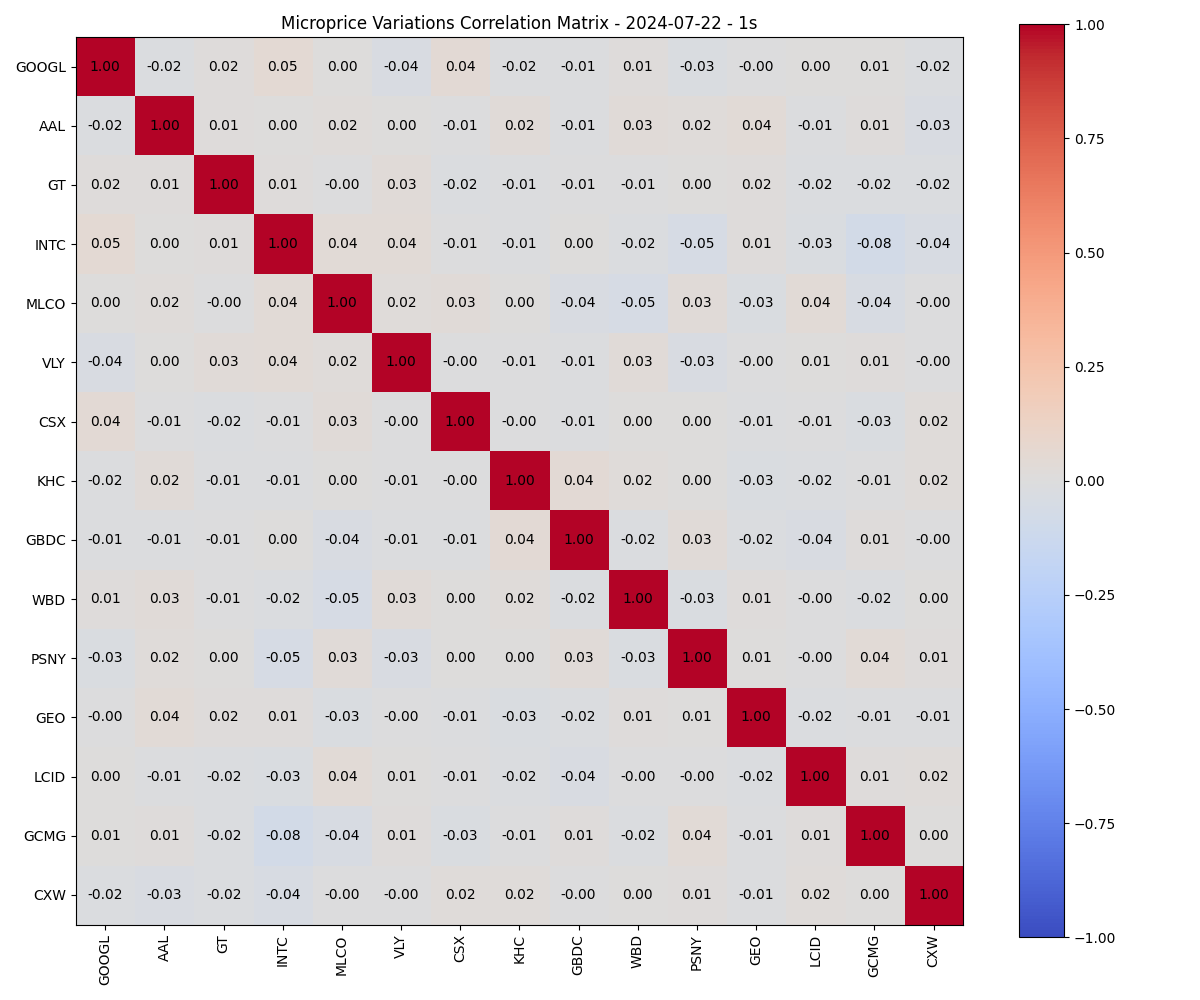
\includegraphics[width=\textwidth]{variations_matrix_2024-07-22_1s.png} % Image prend toute la largeur de la subfigure
        \caption{Échelle 1s}
        \label{fig:corr_1s}
    \end{subfigure}
        \hfill % Espace horizontal flexible
        \begin{subfigure}[b]{0.32\textwidth} % Ajustement de la largeur pour alignement horizontal
            \centering % Centrer l'image dans la subfigure
            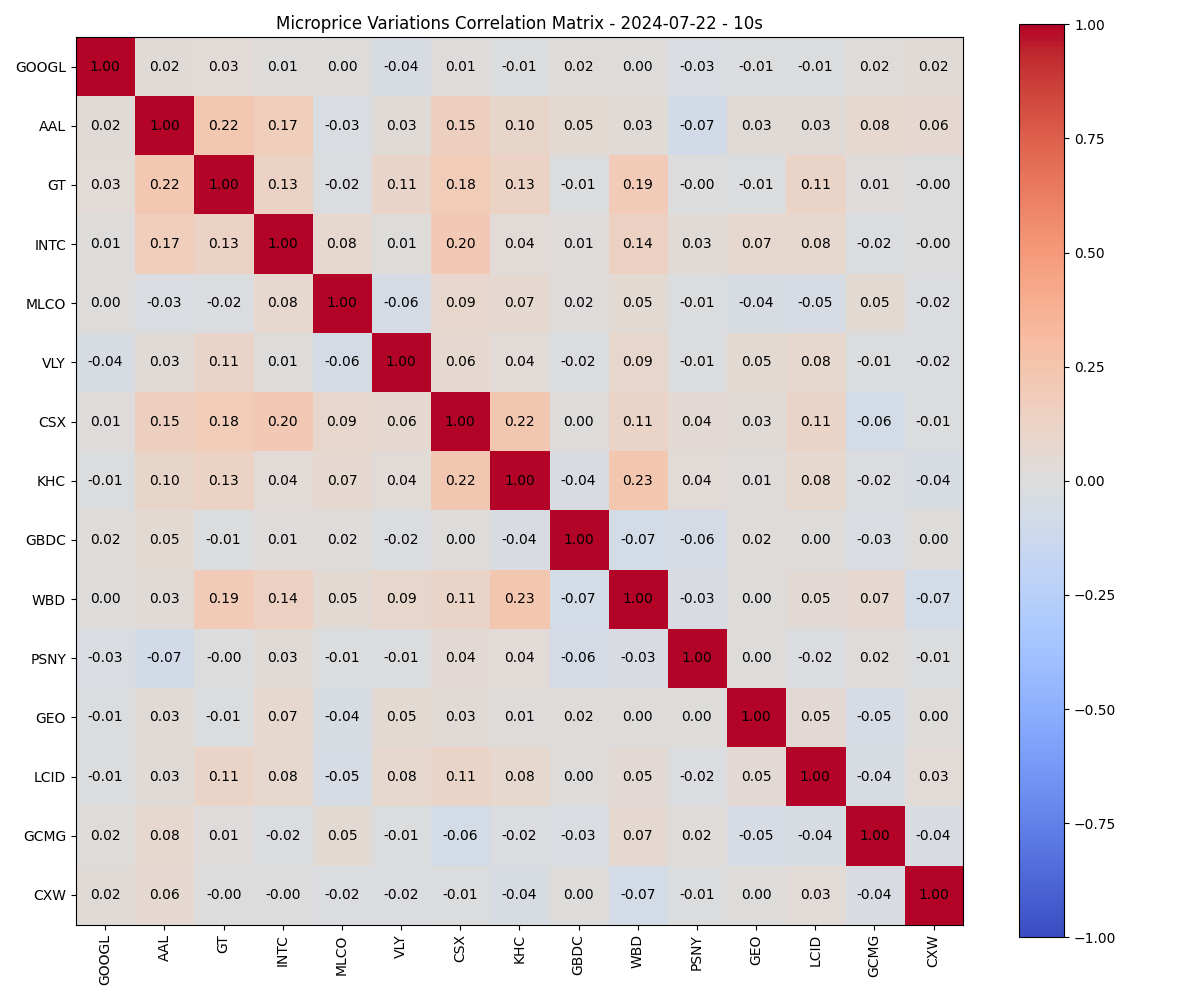
\includegraphics[width=\textwidth]{variations_matrix_2024-07-22_10s.png} % Image prend toute la largeur de la subfigure
        \caption{Échelle 10s}
        \label{fig:corr_10s}
    \end{subfigure}
    \caption{Matrices de corrélation des rendements pour les actifs disponibles le 22 juillet 2024, à différentes échelles temporelles. On observe une augmentation générale des corrélations à mesure que l'échelle de temps s'allonge.}
    \label{fig:correlation_matrices_multiscale}
\end{figure}

Plusieurs observations clés émergent de cette analyse multi-échelle :
\begin{itemize}
    \item \textbf{Échelle microscopique (10ms)} : Les corrélations sont très faibles, proches de zéro pour la plupart des paires. Cela confirme l'indépendance relative des mouvements de prix à très haute fréquence, dominée par le bruit de microstructure.
    \item \textbf{Échelle mésoscopique (1s)} : Les corrélations commencent à émerger, bien que restant modérées. On peut commencer à distinguer certains groupes d'actifs ayant des mouvements légèrement plus synchronisés.
    \item \textbf{Échelle macroscopique (10s)} : Les corrélations sont nettement plus prononcées. Des clusters d'actifs positivement corrélés deviennent visibles, souvent liés à des secteurs d'activité communs (par exemple, technologie, énergie). Les corrélations négatives apparaissent également entre certains groupes. C'est à cette échelle que la structure économique sous-jacente du marché devient la plus apparente dans les corrélations linéaires.
\end{itemize}

Ces résultats soulignent que la structure de dépendance est fortement dépendante de l'échelle. Les corrélations linéaires classiques ne capturent qu'une partie de l'image et sont plus pertinentes aux échelles macroscopiques. Cependant, elles doivent être interprétées avec prudence car :
\begin{itemize}
    \item On ne capture pas les dépendances non-linéaires, particulièrement importantes en période de stress. Cela devient vraiment important en intraday et lors de jumps corrélés sur l'orderbook (voir Hawkes).
    \item Sur plusieurs jours , la structure de corrélation évolue est n'est plus cantonnée à la dynamique intraday. Ces recherches seront à poursuivre dans le futur.
    \item Et donc les actifs qui présentent de faibles corrélations en temps normal (il y en a beaucoup ici) peuvent converger pendant les crises (phénomène de *correlation breakdown*). On étudiera aussi ça dans le futur.
\end{itemize}


On passe maintenant à une analyse plus poussée des dépendances des assets en modélisant la structure de dépendance des returns par des copules.


\section{Analyse des dépendances par les copules}

\subsection{Théorie des copules}

La théorie des copules permet d'étudier les dépendances entre variables aléatoires via le théorème de Sklar : $F(x_1, \ldots, x_n) = C(F_1(x_1), \ldots, F_n(x_n))$ où $F$ est la distribution jointe, $F_i$ les marginales et $C$ la copule. Nous étudions trois copules : Clayton (dépendance queue inférieure), Frank (dépendance symétrique) et Gumbel (dépendance queue supérieure).


\subsection{Résultats empiriques}

L'analyse des copules révèle plusieurs caractéristiques importantes des dépendances entre actifs :

    \begin{itemize}
    \item \textbf{Échelle temporelle} : La force de la dépendance augmente généralement avec l'échelle temporelle, mais atteint un plateau vers 100ms.
    
    \item \textbf{Sélection de modèle} : La copule de Clayton s'avère donc la plus adaptée pour les jours baissiers type 1 Aout 2024, sinon celle de Frank est vraiment adaptée pour les jours sans news type le graphe du dessous.
    
    \item \textbf{Mesures de dépendance} :
    \begin{itemize}
        \item Tau de Kendall : $\tau \in [-0.05, 0.05]$
        \item Rho de Spearman : $\rho \in [-0.05, 0.05]$
        \item Coefficient de queue inférieure : $\lambda_L \in [0.10, 0.35]$
    \end{itemize}
\end{itemize}

\begin{figure}[h!]
\centering
    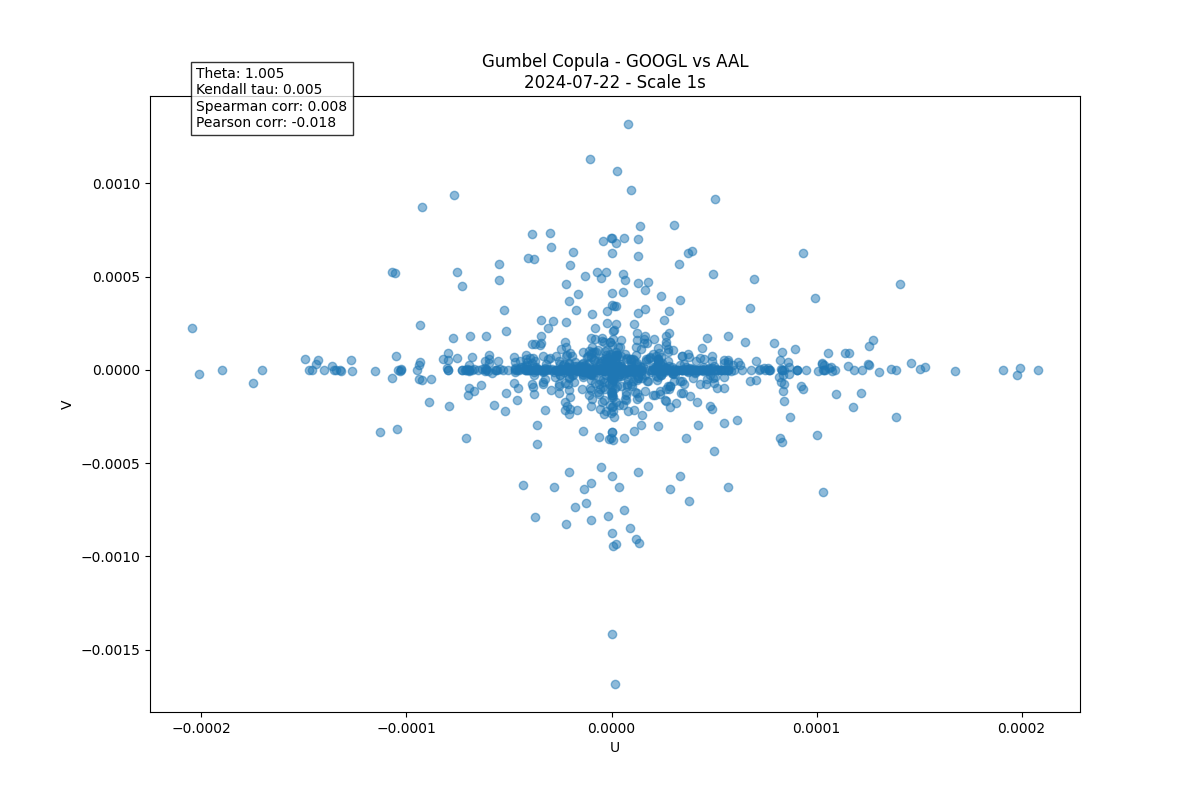
\includegraphics[width=0.8\textwidth]{GOOGL_AAL_2024-07-22_1s.png}
    \caption{Copule de Gumbel estimée pour la paire GOOGL-AAL le 22 juillet 2024 à l'échelle 1s. Jour de news baissier de GOOGL Les paramètres estimés montrent une faible dépendance ($\theta = 1.005$, $\tau = 0.005$), cohérente avec l'hypothèse d'indépendance conditionnelle à haute fréquences sur des jours baissiers avec des stocks dans des secteurs différents.}
    \label{fig:copula_example_app1}
\end{figure}




\subsection{Synthèse des analyses de dépendance et stationnarité}

On peut tirer une conclusion importante sur la nature des dépendances HFT, qui est l'indépendance conditionnelle forte à l'échelle micro, confirmée par la faiblesse des dépendances capturées par les copules à ces échelles ($\tau < 0.2$ pour $\Delta t < 1\text{ms}$).
    
    
On souligne donc l'importance d'une approche multi-échelle dans l'analyse des marchés haute fréquence. C'est le coeur de l'analyse fat-tail, que l'on peut retrouver dans le noyau d'excitation Hawkes dans la suite du rapport. La partie suivante sur les processus de Hawkes reste cependant facultative dans le cadre de ce premier rapport. Nous avons tenté de nous inspirer des travaux de \cite{bacry2014estimationslowlydecreasinghawkes} pour l'estimation des noyaux de Hawkes, mais la librairie standard `tick` n'étant plus maintenue, nous avons dû recoder entièrement la procédure d'estimation non-paramétrique (disponible sur le dépôt GitHub dans `models/hawkes/`). Les premiers essais, lancés sur CUDA en raison du volume de données considérable, sont en cours d'analyse durant le mois d'avril. Bien que cette tâche soit ambitieuse pour ce projet personnel à long terme, les résultats préliminaires sont prometteurs malgré les défis calculatoires rencontrés.


Pour approfondir l'analyse des dépendances temporelles et de la nature des événements extrêmes (sauts), on s'inspire des travaux de Marcaccioli et al. \cite{marcaccioli2021exogenous} qui utilisent des processus de Hawkes pour modéliser et classifier les sauts de prix.


\newpage
\section{Modélisation par processus de Hawkes}

    Pour approfondir l'analyse des dépendances temporelles et de la nature des événements extrêmes (sauts), On s'inspire des travaux de Marcaccioli et al. \cite{marcaccioli2021exogenous} qui utilisent des Hawkes pour modéliser et classifier les sauts de prix.

    \subsection{Le modèle de Hawkes auto-excité}

    Le modèle de Hawkes est un processus ponctuel qui permet de capturer l'auto-excitation, c'est-à-dire le fait qu'un événement augmente la probabilité d'événements futurs. Dans le contexte financier, cela modélise l'idée que des mouvements de prix (ou d'autres événements de marché comme les ordres) peuvent en déclencher d'autres, créant des cascades ou des clusters d'activité.

    L'intensité conditionnelle $\lambda(t)$ du processus, qui représente le taux instantané d'événements à l'instant $t$, est donnée par \cite{marcaccioli2021exogenous} :
    \begin{equation}
    \lambda(t) = \lambda_0(t) + \sum_{t_i < t} \phi(t-t_i)
    \end{equation}
    où :
\begin{itemize}
        \item $\lambda_0(t)$ est l'intensité de base (ou exogène), représentant le taux d'événements déclenchés par des facteurs externes au processus lui-même (par exemple, des nouvelles macroéconomiques non spécifiques).
        \item La somme porte sur tous les événements passés $t_i < t$.
        \item $\phi(\tau)$ est le noyau de mémoire (ou noyau d'excitation), qui quantifie l'influence d'un événement passé sur l'intensité présente. Un $\phi(\tau)$ positif signifie que les événements passés augmentent la probabilité d'événements futurs.
\end{itemize}

    L'article \cite{marcaccioli2021exogenous} explore particulièrement le cas où le noyau de mémoire suit une loi de puissance, $\phi(\tau) \sim 1/\tau^{1+\theta}$ avec $0 < \theta < 1$, typique des systèmes proches de la criticalité. Ce type de noyau à mémoire longue est crucial pour modéliser la persistance observée dans la volatilité et l'activité des marchés. On a vu précedemment que les inter-arrivées suivent précisément une fat-tail conséquente à ce noyau
    
    Un intérêt majeur de ce cadre est sa capacité potentielle à distinguer les sauts de nature différente en analysant le profil de volatilité autour du saut :
\begin{itemize}
        \item \textbf{Sauts Exogènes (EMC - Efficient Market Class)} : Typiquement associés à des nouvelles externes claires. Le modèle prédit une augmentation abrupte de la volatilité sans précurseur notable, suivie d'une relaxation rapide (décroissance en loi de puissance rapide, $\sim (t-t_j)^{\theta-1}$ puis $\sim (t-t_j)^{-\theta-1}$).
        \item \textbf{Sauts Endogènes (SEC - Self-Exciting Class)} : Émergeant de la dynamique interne du marché. Le modèle prédit une augmentation progressive de la volatilité avant le saut, suivie d'une relaxation plus lente (profil plus symétrique, décroissance en loi de puissance $\sim |t-t_j|^{2\theta-1}$ avant et après le saut).
\end{itemize}
    L'estimation des exposants de ces lois de puissance (notamment $p_r$ pour la relaxation post-saut et $p_l$ pour la croissance pré-saut) permettrait ainsi de classifier les sauts observés.

    \subsection{Détection des sauts et score de saut}

    Pour identifier empiriquement les sauts de prix candidats à cette analyse, l'article \cite{marcaccioli2021exogenous} utilise une méthodologie basée sur la standardisation des rendements. L'idée est de normaliser les rendements pour qu'en l'absence de sauts, leur distribution soit proche d'une loi normale centrée réduite, puis d'identifier les valeurs extrêmes par rapport à cette référence.

    Le "score de saut" $J_t$ est défini comme :
\begin{equation}
    J_t = \frac{r_t}{\sigma_t f_t}
\end{equation}
    où :
    \begin{itemize}
        \item $r_t = \log(m_t / m_{t-1})$ est le rendement logarithmique du mid-price à l'échelle considérée (1 minute dans l'article).
        \item $\sigma_t$ est une estimation robuste de la volatilité locale, calculée pour éliminer l'influence des sauts eux-mêmes sur l'estimation de la volatilité courante. L'article utilise une estimation basée sur la variation bipower réalisée :
        \[ \sigma^2_t = \frac{\pi}{2 K} \sum_{i=1}^{K} |r_{t-i}| |r_{t-i+1}| \]
        \item $f_t$ est un facteur de périodicité intra-journalière, estimé pour corriger les variations systématiques de la volatilité au cours de la journée (par exemple, la forme en U ou J inversé). L'estimation se fait en deux étapes pour plus de robustesse.
    \end{itemize}

    Sous l'hypothèse nulle d'absence de sauts, la statistique du maximum de $|J_t|$ sur une fenêtre converge vers une loi de Gumbel. Un seuil est alors déterminé en utilisant la théorie des valeurs extrêmes pour identifier les $J_t$ dont l'amplitude est statistiquement improbable (par exemple, avec un seuil de significativité $\alpha$).

    \fbox{\begin{minipage}{0.9\textwidth}
    \textbf{Hyperparamètres typiques de \cite{marcaccioli2021exogenous}:}
    \begin{itemize}[nosep]
        \item Fenêtre de volatilité locale : $K=390$ (minutes, soit 1 jour de trading US)
        \item Seuil de significativité pour la détection de saut : $\alpha = 0.01$ (correspondant à $|J_t| \approx 4.36$)
        \item Échelle d'échantillonnage : 1 minute
    \end{itemize}
    \end{minipage}}

    \subsection{Profils de sauts observés}

    Nous illustrons des profils de sauts typiques observés sur des instants non triviaux, c'est à dire où le jump ne se distingue pas forcément des autres à vue d'oeil mais se voit dans le score, dans nos données, en comparant le cours de l'actif et le score de saut $J_t$.

    \begin{figure}[H]
        \centering
        \includegraphics[width=0.53\textwidth]{Exemple 1.png}
        \caption{Profil de saut pour l'actif AAPL le 2024-10-10 (Exemple 1)}
        \label{fig:jump_example_1}
    \end{figure}
    
    On observe que le comportement du prix (cours de l'action en bleu) et du "jump-score" Jt ne présentent pas de corrélation visuellement évidente. Autour du saut (lorsque le jump-score dépasse 4,36) , on n'observe pas d'évolution locale plus marquée. Concernant le saut en lui-même, il semble être du type exogène (EMC). En effet, la volatilité augmente abruptement, sans précurseur notable, suivi d'une relaxation rapide. On observe une seconde excitation, qui ne dépasse pas le seuil de 4,36, mais qui témoigne de l'existence de paquets d'excitations successives de même nature. 

    \vspace{1cm}

    \begin{figure}[H]
        \centering
        \includegraphics[width=0.53\textwidth]{Exemple 2 better.png}
        \caption{Profil de saut pour l'actif AAPL le 2024-10-10 (Exemple 2)}
        \label{fig:jump_example_2}
    \end{figure}

    Ici, contrairement à l'exemple 1, on observe un saut endogène (SEC). En effet, une excitation graduelle précède le saut. La volatilité décroit plus graduellement après le saut. 
    

    \vspace{1cm}

    \begin{figure}[H]
        \centering
        \includegraphics[width=0.53\textwidth]{MSFT_2024-11-01_xnas-itch.parquet 2024-11-01 10:40:00-04:00Jump and approx.png}
        \caption{Profil de saut pour l'actif MSFT le 2024-11-01 (Exemple 3)}
        \label{fig:jump_example_3}
    \end{figure}
    On tente alors de trouver une régression qui approxime la courbe de "Jump score". Dans l'exemple 3, on est en présence d'un saut d'apparence exogène. On obtient que le saut est bien modélisé par un palier de volatilité (absence de précurseur), suivi d'un saut, puis d'une relaxation rapide (loi de puissance rapide). Le paramètre theta choisi est $\Theta = 0.5$. 

    \vspace{1cm}

    \begin{figure}[H]
        \centering
        \includegraphics[width=0.53\textwidth]{PHOTO-2025-04-01-12-04-48.jpg}
        \caption{Profil de saut pour l'actif AAPL le 2024-10-10 (Exemple 4)}
        \label{fig:jump_example_4}
    \end{figure}

    Enfin, on reprend la situation de la figure 2, et ayant reconnu un saut endogène, on applique le modèle d'un profil symétrique, suivant une loi de puissance sur le voisinage du jump à environ 20 timestamps voisins. On obtient un résultat satisfaisant, la théorie est pour l'instant conforme aux observations.
    
    \subsection{Conclusion sur l'approche}

    \begin{figure}[H]
        \centering
        \includegraphics[width=0.53\textwidth]{AAPL_2024-10-10_xnas-itch.parquet single jumps histogram.png}
        \caption{Histogramme du profil des sauts pour l'actif AAPL le 2024-10-10}
        \label{fig:jump_example_4}
    \end{figure}

    On observe sur cet histogramme un profil qui rappelle à droite du pic une loi puissance, et à gauche également, cependant plus estompée encore par le fait que les sauts exogènes présentent un profil de "jump score" plat avant le saut.
    \vspace{0.3cm}

    La détection des sauts proposée par \cite{marcaccioli2021exogenous} apparaît comme un succès, comme le met en évidence l'histogramme précédent par son unique pic lisible (certes bien choisi, mais la plupart des profils sont ainsi).
    \vspace{0.3cm}

    La classification des sauts en deux catégories semble très pertinente, bien qu'on rencontre deux problèmes : relier les sauts supposés exogènes aux évènements extérieurs, et s'assurer de l'absence d'évènements ayant pu déclencher un saut supposé endogène. En revanche, ce lien entre la microstructure du marché et les évènements externes nous invite à étudier la valeur du $\theta$ que nous n'avons pas encore fitté mais que l'on a déduit à travers les profils de sauts, Les méthodes sont prometteuses et nous les poursuivrons dans les semaines à venir.
    

\newpage
\section*{Conclusion}
    Ce mémoire a initié une exploration statistique approfondie d'un jeu de données haute fréquence LOB du Nasdaq, posant les bases d'une compréhension fine de la microstructure de marché sur plusieurs actifs et échelles temporelles. Nos analyses ont systématiquement validé plusieurs faits stylisés fondamentaux tout en révélant la complexité multi-échelle des dynamiques de prix. Aucun des 3 participants au projet ne suivent un cursus ou stage en finance quantitative, cela était donc l'objet d'une réèlle découverte attisée par notre curiosité du fonctionnement des marchés HFT.

    \vspace{0.5cm}

    L'étude des rendements a confirmé sans équivoque la présence de queues de distribution lourdes, caractérisées par des indices de queue $\alpha$ estimés par la méthode de Hill typiquement entre 2.4 et 3.1. Cette propriété, robuste à travers différents actifs et échelles temporelles (5m à 1h), non seulement quantifie le risque d'événements extrêmes mais valide aussi l'hypothèse cruciale d'intégrabilité $L^2$, légitimant ainsi l'analyse des corrélations. L'analyse de l'exposant de Hurst a révélé une forte anti-persistance (H ≈ 0.23-0.33) aux échelles microscopiques (< 60s), typique des retours rapides vers la moyenne induits par le *bid-ask bounce* et l'activité des *market makers*, tandis que l'autocorrélation des rendements a mis en évidence une mémoire longue, signe d'une volatilité persistante et agrégée.

    \vspace{0.5cm}

    L'analyse de la stationnarité, via les tests ADF et la détection de ruptures, a montré que si les séries de prix sont localement non-stationnaires à très haute fréquence (100ms), elles peuvent être considérées comme stationnaires par morceaux sur des échelles plus longues (1s-60s). Ces ruptures de stationnarité coïncident souvent avec des événements macroéconomiques majeurs, induisant des réactions synchronisées sur l'ensemble des actifs, même ceux évoluant dans des secteurs différents. Ce phénomène souligne l'interaction complexe entre les dynamiques endogènes rapides et les chocs exogènes.

    \vspace{0.5cm}

    La structure de dépendance, explorée par les matrices de corrélation linéaire et les copules, s'est également avérée fortement dépendante de l'échelle. Une indépendance quasi-totale aux échelles microscopiques (10ms) laisse place à des structures de corrélation plus marquées (clusters sectoriels) et à une dépendance non-linéaire (souvent capturée par la copule de Clayton, indiquant une dépendance accrue lors des baisses) aux échelles de la seconde et au-delà. Cette observation, couplée à la synchronisation des ruptures lors d'événements externes, suggère que si le bruit de microstructure domine à très court terme, les facteurs communs et les interactions systémiques deviennent prépondérants lorsque l'horizon temporel s'allonge.

    \vspace{0.5cm}

    Ces résultats empiriques s'inscrivent bien dans le cadre théorique des processus auto-excités comme les processus de Hawkes, et de la distinction de Bouchaud entre sauts endogènes (SEC), majoritaires et liés à la dynamique interne du LOB (reflétée par l'anti-persistance et les queues lourdes des temps d'arrivée), et sauts exogènes (EMC), plus rares mais synchronisés et liés aux informations externes. L'ensemble de ce travail préliminaire de caractérisation statistique ouvre ainsi la voie à une modélisation plus fine intégrant ces différentes facettes, notamment en reliant les modèles de volatilité rough aux processus de Hawkes sous-jacents pour capturer la dynamique multi-échelle complexe des marchés financiers.

    \vspace{0.5cm}

    Nous avons finalement remarqué qu'aucune librairie python open-source ne permettait de bien fitter un modèle de Hawkes (tick, pyhawkes, Hawkes et hawkeslib), nous continuerons notre projet en construisant une librairie open-sourcée qui permettra de s'accorder sur une estimation efficace sur des données quelconques (sismiques ou populations) et HFT (voir librarie tick qui n'est plus maintenue).

\newpage
\begin{thebibliography}{9}

\bibitem{chong2024minimax}
Carsten Chong, Marc Hoffmann, Yanghui Liu, Mathieu Rosenbaum, and Grégoire Szymanski.
\newblock Statistical inference for rough volatility: Minimax Theory.
\newblock \emph{arXiv preprint arXiv:2210.01214}, 2024.
\newblock URL: \url{https://arxiv.org/abs/2210.01214}.

\bibitem{chong2024clt}
Carsten H. Chong, Marc Hoffmann, Yanghui Liu, Mathieu Rosenbaum, and Grégoire Szymanski.
\newblock Statistical inference for rough volatility: Central limit theorems.
\newblock \emph{The Annals of Applied Probability}, 34(3), 2024.
\newblock DOI: \href{http://dx.doi.org/10.1214/23-AAP2002}{10.1214/23-aap2002}.

\bibitem{marcaccioli2021exogenous}
Riccardo Marcaccioli, Jean-Philippe Bouchaud, and Michael Benzaquen.
\newblock Exogenous and endogenous price jumps belong to different dynamical classes.
\newblock \emph{Journal of Statistical Mechanics: Theory and Experiment}, 2022(2):023403, 2022.
\newblock DOI: \href{http://dx.doi.org/10.1088/1742-5468/ac498c}{10.1088/1742-5468/ac498c}.

\bibitem{bacry2014estimationslowlydecreasinghawkes}
Emmanuel Bacry, Thibault Jaisson, and Jean-Francois Muzy.
\newblock Estimation of slowly decreasing Hawkes kernels: Application to high frequency order book modelling.
\newblock \emph{arXiv preprint arXiv:1412.7096}, 2014.
\newblock URL: \url{https://arxiv.org/abs/1412.7096}.

\bibitem{saddier2024bayesiantheorymarketimpact}
Louis Saddier and Matteo Marsili.
\newblock A Bayesian theory of market impact.
\newblock \emph{arXiv preprint arXiv:2303.08867}, 2024.
\newblock URL: \url{https://arxiv.org/abs/2303.08867}.

\end{thebibliography}

\end{document}